\chapter{Cenni alla misura di Lebesgue}
\pagestyle{plain}
\thispagestyle{empty}
\pagestyle{fancy}
In questo capitolo affronteremo il concetto di misura e daremo alcuni accenni all'impostazione teorica data da Lebesgue nello sviluppo
del suo concetto di misura. Alcuni approfondimenti inseriti sono stati presi da \cite{rudin} oppure \cite{tao}. Per una trattazione completa e, naturalmente, rigorosa consiglio un testo molto famoso della materia, ovvero \cite{measure_theory}.

\section{La misura esterna}
Vogliamo adesso determinare una funzione di insiemi $m_n: \mathcal{P}(\mathbb{R}^n) \to [0; +\infty]$ che rappresenta il nostro concetto intuitivo di \emph{volume} dell'insieme, detto \emph{misura dell'insieme}. \\
L'intuizione ci porta a pensare che questa funzione goda delle seguenti proprietà:
\begin{enumerate}[label=\protect\circled{\arabic*}]
	\item $m_n(\emptyset) = 0$
	\item Se $A, B \subseteq X$ tali che $A \subseteq B \implies m_n(A) \leq m_n(B)$
	\item Se $A, B \subseteq X$ tali che $A \cap B = \emptyset \implies m_n(A \cup B) = m_n(A) + m_n(B)$
\end{enumerate}
Prima di procedere ulteriormente sullo sviluppo della teoria della misura di Lebesgue, vorrei aprire una breve parentesi "qualitativa" su come trovare la misura di un insieme: l'approccio più \emph{naive} possibile consiste nel coprire il nostro insieme con dei rettangoli e sommare i volumi di questi rettangoli. Questo approccio ci consente di ottenere quello che viene chiamata \emph{misura esterna}, ovvero una funzione d'insieme che è ben definita su ogni insieme e che soddisfa tutte le buone
proprietà che ci aspettiamo da una misura che generalizza il nostro concetto di misura tranne quella di additività della misura. Per essere una misura "vera e propria" (ovvero che goda anche di additività) si può mostrare che è necessario restringerci
ad una classe di insiemi (che saranno gli insiemi \emph{misurabili}) su cui la nostra misura esterna godrà di additività (questo risultato prende il nome di \emph{teorema di Caratheodory}, di cui non daremo dimostrazione).
\begin{definition}[misura di un intervallo e di un $n-$intervallo]
	Per ogni intervallo $I \subseteq \mathbb{R}$ limitato definiamo
	$$
	\mathit{l}(I) = \sup{I} - \inf{I}.
	$$
	Sia adesso $I_1 \times \ldots \times I_n \subseteq \mathbb{R}^n$ definiamo
	$$
		v_n \left( \varprod_{i=1}^n I_i \right) = \prod_{i=1}^n \mathit{l}(I_i) 
	$$
\end{definition}
\begin{definition}[misura di Lebesgue di un insieme $E$]
	Sia $E \subseteq \mathbb{R}^n$, definiamo la misura di Lebesgue di $E$ come
	\begin{equation}
		m_n(E) = \inf \left\{ \sum_{i=1}^{+\infty} v_n(J_i) : E \subseteq \bigcup_{i=1}^{+\infty} J_i \text{ e } J_i \subseteq \mathbb{R}^n \text{ è un } n\text{-intervallo} \right\}
		\label{eq:def_lebesgue}
	\end{equation}
\end{definition}
\begin{definition}
	Diremo che $\mu^*: \mathcal{P}(X) \mapsto [0; +\infty]$ è una misura esterna se
	\begin{enumerate}[label=\protect\circled{\arabic*}]
		\item $\mu^*(\emptyset) = 0$;
		\item $\mu^*(E) \leq \sum\limits_{i=1}^{+\infty} \mu^*(E_i)$ se $E \subseteq \bigcup\limits_{i=1}^{+\infty} E_i$
	\end{enumerate}
\end{definition}
\begin{prop}[monotonia della misura esterna]
	Se $\mu^*$ è una misura esterna allora
	$$
	A \subseteq B \implies \mu^*(A) \leq \mu^*(B)
	$$
	\label{prop:monotonia}
\end{prop}
\begin{proof}
	Consideriamo $E = A$ e il seguente insieme
	\begin{align*}
	E_j = \begin{cases} B & j=1 \\ \emptyset & j \geq 2	\end{cases}
	\end{align*}
	osserviamo allora che $E \subseteq \bigcup\limits_{i=1}^{+\infty} E_i$ allora
	$$
	\mu^*(E) = \mu^*(A) \stackrel{\text{per la \circled{2}}}{\leq} \sum_{j=1}^{+\infty} \mu^*(E_j) = \mu^*(E_1) = \mu^*(B)
	$$
	ovvero
	$$
	\mu^*(A) \leq \mu^*(B)
	$$
\end{proof}
\begin{prop}[subadditività finita]
	Le misure esterne sono finitamente subadditive, ovvero preso $E_1, \ldots, E_k$ avremo che 
	$$
	\mu^* \left( \bigcup_{i=1}^{k} E_i \right) \leq \sum_{i=1}^k \mu^*(E_i)
	$$
	\label{prop:sub_finita}
\end{prop}
\begin{proof}
	Siano $E_1, \ldots, E_k \subseteq \mathbb{R}^n$. Imponendo che $\forall j > k, E_j = \emptyset$, allora
	$$
	\forall E \subseteq \bigcup_{i=1}^{+\infty} E_i, \mu^*(E) \leq \sum_{i=1}^{+\infty} \mu^*(E_i) = \sum\limits_{i=1}^{k} \mu^*(E_i) + \sum\limits_{i=k+1}^{+\infty} \mu^*(\emptyset) = \sum\limits_{i=1}^k \mu^*(E_i) \implies \mu^*(E) \leq \sum_{i=1}^k \mu^*(E_i)
	$$
	ma allora, siccome abbiamo banalmente che $\bigcup\limits_{i=1}^{k} E_i \subseteq \bigcup\limits_{i=1}^k E_i$, allora
	$$
	\mu^* \left( \bigcup_{i=1}^k E_i \right) \leq \sum_{i=1}^k \mu^*(E_i)
	$$
\end{proof}
Vogliamo adesso mostrare che la funzione d'insieme $m_n$ da noi definita è effettivamente una misura esterna, dunque, in virtù di quanto detto, possiamo individuare e restringere $m_n$ ad una classe di insiemi per cui $m_n$ rappresenta una vera e propria misura.
\begin{prop}[misura di Lebesgue è una misura esterna]
	$m_n: \mathcal{P}(X) \to [0; +\infty]$ è una misura esterna
	\label{prop:lebesgue_mis_esterna}
\end{prop}
\begin{proof}
	La dimostrazione consiste nel mostrare che $m_n: \mathcal{P}(X) \mapsto [0; +\infty]$ gode delle proprietà della misura esterna. \\
	La \circled{1} segue banalmente, siccome l'$n-$intervallo nullo è un ricoprimento dell'insieme nullo, dunque $m_n(\emptyset) = 0$.
	Per la \circled{2}, supponiamo naturalmente che $\sum\limits_{i=1}^{+\infty} m_n(E_i) < +\infty$ (altrimenti è banale) e prendiamo un insieme $E \subseteq \bigcup\limits_{i=1}^{+\infty} E_i$, osservando che $\forall i \in \mathbb{N}, E_i \subseteq \bigcup\limits_{k=1}^{+\infty} I_{k}^{(i)}$, pertanto
	$$
		E \subseteq \bigcup_{i=1}^{+\infty} \bigcup_{k=1}^{+\infty} I_k^{(i)}
	$$
	e questo vale per ogni ricoprimento di $\bigcup\limits_{i=1}^{+\infty} E_i$, dunque anche per quello che "fornisce" la misura di $\bigcup\limits_{i=1}^{+\infty} E_i$
	$$
		m_n(E) \leq \inf \left\{\sum_{i=1} l(E_i) \right\} = m_n \left( \bigcup_{i=1}^{+\infty} E_i \right)
	$$
	resta da mostrare che $m_n( \bigcup\limits_{i=1}^{+\infty} E_i ) \leq \sum\limits_{i=1}^{+\infty} m_n(E_i)$ . Questo può essere fatto fissando $\varepsilon > 0$ e osservando che $\forall i \in \mathbb{N}, \exists \bigcup\limits_{k=1}^{+\infty} I_{i}^{(k)} \supseteq E_i : \sum\limits_{k=1}^{+\infty} l(I_i^{(k)}) < m_n(E_i) + \frac{\varepsilon}{2^{i+1}}$, dunque
	$$
	m_n \left( \bigcup_{i=1}^{+\infty} E_i \right) \leq \sum_{i=1}^{+\infty} \sum_{k=1}^{+\infty} l(I_{i}^{(k)}) < \sum_{i=1}^{+\infty} (m_n(E_i) + \frac{\varepsilon}{2^{i+1}}) = \varepsilon + \sum_{i=1}^{+\infty} m_n(E_i)
	$$
	e, siccome $\varepsilon$ era arbitrario, otteniamo la tesi facendo il limite.
\end{proof}
\begin{definition}[insieme misurabile secondo Lebesgue]
	Diremo che $A \subseteq X$ è misurabile secondo Lebesgue se
	$$
	\forall S \subseteq X \implies m_n(S) = m_n(A \cap S) + m_n(S \setminus A)
	$$
	\label{def:mis_lebesgue}
\end{definition}
Per ogni insieme $X$ definiamo con $\mathfrak{M}(X)$ la classe di tutti gli insiemi misurabili secondo Lebesgue.
\begin{definition}[$\sigma-$algebra]
	Diremo che $\mathcal{F} \subseteq \mathcal{P}(X)$ è una $\sigma-$algebra se valgono
	\begin{enumerate}[label=\protect\circled{\arabic*}]
		\item $\emptyset, X \in \mathcal{F}$;
		\item $A \in \mathcal{F} \implies (X \setminus A) \in \mathcal{F}$
		\item $\{ A_j : j \geq 1 \} \subseteq \mathcal{F} \implies \bigcup\limits_{i=1}^{+\infty} A_i \in \mathcal{F}$
	\end{enumerate}
\end{definition}
\begin{definition}[misura]
	Diremo che $\mu: \mathcal{F} \mapsto [0; +\infty]$ è una misura se
	\begin{enumerate}[label=\protect\circled{\arabic*}]
		\item $\mathcal{F}$ è una $\sigma-$algebra;
		\item $\mu(\emptyset) = 0$;
		\item Se $( \{A_i : i \geq 1 \} \subseteq \mathcal{F}) \wedge (\forall i \neq j, A_i \cap A_j = \emptyset$) allora
		$$
			\mu \left( \bigcup_{i=1}^{+\infty} A_i \right) = \sum_{i=1}^{+\infty} \mu(A_i)
		$$
	\end{enumerate}
\end{definition}
\begin{theorem}
	La classe dei misurabili $\mathfrak{M}(X)$ è una $\sigma-$algebra e $m_n:\mathfrak{M}(X) \to [0; +\infty]$ è una misura
\end{theorem}
Diremo allora che $m_n: \mathfrak{M}(X) \to [0; +\infty]$ è la misura di Lebesgue su $X$. Per lo più noi lavoreremo supponendo che $X=\mathbb{R}^n$.
\begin{prop}
	La misura $m_n: \mathfrak{M}(X) \to [0; +\infty]$ è finitamente additiva
\end{prop}
\begin{proof}
La dimostrazione è equivalente a quella della proposizione~\ref{prop:sub_finita} sostituendo opportunamente alle minorazione le eguaglianze.
\end{proof}
\begin{remark}
Ammettendo l'assioma della scelta è possibile mostrare che esistono degli insiemi che non sono misurabili (come ampiamente detto in precedenza). L'esempio più famoso è
l'insieme di Vitali, che si può costruire dentro un qualunque insieme di misura positiva $E \in \mathfrak{M}(\mathbb{R}^n)$. Dalla definizione di misurabilità allora $\exists S_0 \subseteq \mathbb{R}^n$
tale che 
$$
m_n(S_0) \leq m_n(S_0 \cap E) + m_n(S_0 \setminus E)
$$
dunqque si perderebbe la $\sigma-$additività su insiemi disgiunti.
\end{remark}
\subsection{Insiemi trascurabili}
\begin{definition}[insiemi trascurabili]
	Diremo che $Z \subseteq \mathbb{R}^n$ ha misura nulla oppure che è trascurabile se $m_n(Z) = 0$
\end{definition}
\begin{exercise}
	Mostrare che un punto $x \in \mathbb{R}^n$ ha misura nulla
\end{exercise}
\begin{proof}[Svolgimento]
	Sia $x \in \mathbb{R}^n$ e consideriamo un $n-$intervallo $\varprod\limits_{i=1}^n I_i$ dove $I_i = (x_i - \frac{\varepsilon}{2}, x_i + \frac{\varepsilon}{2})$ ($x_i$ rappresenta la $i-$esima componente del punto $x$), dunque rappresenta un cubo di \emph{volume} pari a $\varepsilon^n$ per $i \in \{1, \ldots, n \}$ con $\varepsilon > 0$. Allora possiamo osservare che
	$$
	\{ x \} \subseteq \bigcup_{i=1}^{+\infty} J_i
	$$
	dove
	\begin{align*}
		J_i = \begin{cases}
			\varprod_{i=1}^n (x_i - \frac{\varepsilon}{2}, x_i + \frac{\varepsilon}{2}) \\
			\emptyset
		\end{cases}
	\end{align*}
	ma allora
	$$
	m_n(\{ x \}) \subseteq \bigcup_{i=1}^{+\infty} v_n(J_i) = \varepsilon^n
	$$
	ma allora, siccome $\varepsilon > 0$ è un valore arbitrario, possiamo farne il limite per $\varepsilon \to 0$, dunque $m_n(\{ x \}) = 0$.
\end{proof}
\begin{prop}
	Se $Z \subseteq \mathbb{R}^n$ è numerabile, allora
	$$
		m_n(Z) = 0
	$$
\end{prop}
\begin{remark}
	Non tutti gli insiemi a misura nulla sono numerabili: un esempio è l'insieme di Cantor.
\end{remark}
\begin{proof}
	Se $Z$ è numerabile allora
	$$
		Z = \bigcup_{i=1}^{+\infty} \{ x_i \}
	$$
	dove $x_i: \mathbb{N} \to Z$ dunque
	$$
	m_n(Z) \leq \sum_{i=1}^{+\infty} m_n(\{ x_i \}) = 0 \implies m_n(Z) = 0
	$$
\end{proof}
\begin{cor}
	$\mathbb{Q}^n$ è un insieme trascurabile
\end{cor}
\begin{proof}
$\mathbb{Q}^n \cong \mathbb{N}$ dunque $m_n(\mathbb{Q}^n) = 0$
\end{proof}
\begin{cor}
	Gli insiemi a misura nulla sono misurabili per Lebesgue.
	\label{cor:mis_nulla_misur}
\end{cor}
\begin{proof}
In virtù della definizione~\ref{def:mis_lebesgue} dobbiamo verificare che, preso $Z$ insieme trascurabile, allora
$$
\forall S \subseteq \mathbb{R}^n, m_n(S) = m_n(S \setminus Z) + m_n(S \cap Z)
$$
Ora osserviamo che, siccome $S = (S \setminus Z) \cup (S \cap Z)$, avremo per la subadditività finita (di cui gode $m_n$ siccome nella proposizione~\ref{prop:lebesgue_mis_esterna} abbiamo mostrare che è una misura esterna)
che
$$
m_n(S) \leq m_n(S \setminus Z) \cup (S \cap Z)
$$
Per la disuguaglianza opposta osserviamo che
\begin{align*}
m_n(S) \geq m_n(S \setminus Z) \text{ e } m_n(Z) \geq m_n(S \cap Z)
\end{align*}
per monotonia della misura esterna (proposizione~\ref{prop:monotonia}), ma siccome $0=m_n(Z) \geq m_n(S \cap Z) \implies m_n(S \cap Z) = 0$ allora
$$
m_n(S) \geq m_n(S \setminus Z) = m_n(S \setminus Z) + m_n(S \cap Z) \implies m_n(S) \geq m_n(S \setminus Z) + m_n(S \cap Z)
$$
dunque $m_n(S) = m_n(S \setminus Z) + m_n(S \cap Z)$, ovvero la tesi.
\end{proof}
\begin{theorem}[gli aperti sono misurabili]
	Tutti gli aperti di $\mathbb{R}^n$ sono misurabili secondo Lebesgue
\end{theorem}
Per dimostrare questo teorema abbiamo bisogno del seguente lemma:
\begin{lemma}
Ogni aperto di $\mathbb{R}^n$ è unione numerabile di $n-$intervalli a due a due disgiunti
\end{lemma}
\begin{proof}
	Sia $A \subseteq \mathbb{R}^n$ aperto non vuoto. Allora possiamo considerare la famiglia degli $n-$intervalli $I \subseteq A$ ad estremi razionali, ovvero:
	$$\mathcal{V} = \{I = \prod_{i=1}^n (a_i, b_i] : I \subseteq A, a_i, b_i \in \mathbb{Q} \, \, \forall i \in \{1, \ldots, n\} \}$$
	Siccome ogni $n-$intervallo all'interno di $\mathcal{V}$ può essere messo in corrispondenza biunivoca con la $2n-$upla $(a_1, \ldots, a_n, b_1, \ldots, b_n) \in \mathbb{Q}^{2n}$ che è un insieme numerabile, allora anche $\mathcal{V}$ è un insieme numerabile. E' banale l'inclusione $\bigcup\limits_{I \in A} I \subseteq A$ (per definizione di $\mathcal{V}$), vogliamo
	adesso mostrare che vale anche l'inclusione opposta: sia $x \in A$ e, siccome $A$ è aperto, avremo che 
	$$\forall y \in A, \exists \varepsilon > 0 : \{y = (y_1, \ldots, y_n) \in \mathbb{R}^n : |y_i - x_i| < \varepsilon \, \, \forall i \in \{1, \ldots, n \} \} \subseteq A$$
	Siccome $\mathbb{Q}$ è denso in $\mathbb{R}$ avremo che $\forall i \in \{1, \ldots, n \}, \exists \alpha_i, \beta_i \in \mathbb{Q}$ tali che
	$$
	x_i - \varepsilon < \alpha_i < x_i < \beta_i < x_i + \varepsilon 
	$$
	Dunque avremo che l'$n-$intervallo $I'=\prod\limits_{i=1} (\alpha_i, \beta_i]$ contiene il punto $x$, dunque $x \in \mathcal{V} \implies x \in \bigcup\limits_{I \in \mathcal{V}} I \implies A \subseteq \bigcup\limits_{I \in \mathcal{V}} I$. Concludiamo
	che $A = \bigcup\limits_{i=1} I$. \\
	Mostriamo adesso che possiamo prendere gli $n-$intervalli a due a due disgiunti. Consideriamo $A = \bigcup\limits_{i=i}^{+\infty} I_i$ ma allora, posto $J_i = I_i \setminus \bigcup\limits_{j=1}^{i-1} I_j$, possiamo vedere facilmente che
	$$
	\bigcup_{i=1}^{+\infty} I_i = \bigcup_{i=1}^{+\infty} J_i = A
	$$
\end{proof}
Siamo pronti adesso a dimostrare il teorema:
\begin{proof}[Dimostrazione (del teorema)]
	Sia $A$ un insieme aperto. Per il lemma precedente sappiamo che $A = P = \bigcup\limits_{k=1}^{+\infty} I_i$ dove $I_i$ è un $n-$intervallo, dunque $m_n(P \setminus A) = m_n(\emptyset) = 0$.
	Pertanto $P \setminus A \in \mathfrak{M}(\mathbb{R}^n)$ e $P \in \mathfrak{M}(\mathbb{R}^n)$ siccome unione di $n-$intervalli. 
\end{proof}
\begin{cor}
	Tutti gli insiemi chiusi di $\mathbb{R}^n$ sono misurabili secondo Lebesgue
\end{cor}
\begin{proof}[Dimostrazione (del corollario)]
	Siccome $m_n: \mathfrak{M}(\mathbb{R}^n) \to [0; +\infty]$ allora $\mathfrak{M}(\mathbb{R}^n)$ è una $\sigma-$algebra, dunque se $A \in \mathfrak{M}(\mathbb{R}^n) \implies A^c \in \mathfrak{M}(\mathbb{R}^n)$.
\end{proof}
\begin{cor}
	Tutte le unioni e le intersezioni numerabili di insiemi chiusi o aperti sono ancora misurabili secondo Lebesgue
\end{cor}
\begin{proof}
	Se $\{ B_i : i \geq 1 \} \subseteq \mathfrak{M}(\mathbb{R}^n) \implies \bigcup\limits_{i=1}^{+\infty} B_i \in \mathfrak{M}(\mathbb{R}^n)$ perché $\mathfrak{M}(\mathbb{R}^n)$ è una $\sigma-$algebra, mentre per le intersezioni numerabili abbiamo che se $B_i \in \mathfrak{M}(\mathbb{R}^n) \implies B_i^c \in \mathfrak{M}(\mathbb{R}^n)$ (sempre per le proprietà delle $\sigma-$algebre)
	e, per le leggi di De Morgan, avremo che $\left(\bigcup\limits_{i=1}^{+\infty} B_i^c \right)^c = \bigcap\limits_{i=1}^{+\infty} B_i \in \mathfrak{M}(\mathbb{R}^n)$
\end{proof}
\section{Funzioni misurabili secondo Lebesgue}
Andiamo adesso ad affrontare il concetto di funzione misurabile, il quale ci condurrà, naturalmente, verso il concetto di integrale di Lebesgue
\begin{definition}[funzioni misurabili secondo Lebesgue]
Sia $E \in \mathfrak{M}(\mathbb{R}^n)$ misurabile e $f: E \to \bar{\mathbb{R}}$. Diremo che $f$ è misurabile secondo Lebesgue se $\forall t \in \mathbb{R}$ l'insieme $f^{-1}([-\infty, t)) \in \mathfrak{M}(\mathbb{R}^n)$, ovvero esso è misurabile.
\end{definition}
\begin{remark}(\textbf{Topologia di $[-\infty, \infty]$})
	Ogni aperto di $[-\infty, +\infty]$ è un'unione arbitraria di intervalli che possono essere sia aperti oppure del tipo $[-\infty, t)$ o $(t, +\infty]$.
\end{remark}
\begin{prop}[caratterizzazione delle funzioni misurabili]
	$E \in \mathfrak{M}(\mathbb{R}^n), f: E \to \bar{\mathbb{R}}$ è misurabile se e solo se $\forall O \subseteq \bar{\mathbb{R}}$ aperto di $[-\infty, +\infty]$ abbiamo che $f^{-1}(O) \in M(\mathbb{R}^n)$
\end{prop}
\begin{prop}[le funzioni continue sono misurabili]
	Se $E \in \mathcal{R}^n, f: E \to \mathbb{R}$ è continua, allora è misurabile
\end{prop}
\begin{proof}
	Se $O \subseteq [-\infty, +\infty]$ è un aperto contenuto in $\mathbb{R}$ in realtà è un aperto di $\mathbb{R} \implies f^{-1}(O)$ è aperto in $E$ in virtù del teorema~\ref{thm:teo_cf1}, dunque avremo che $\exists \Omega \subseteq \mathbb{R}^n$ tale che
	$$
	f^{-1}(0) = E \cap \Omega \in \mathfrak{M}(\mathbb{R}^n) \implies f \text{ è misurabile }
	$$
	ovvero la tesi.
\end{proof}
\begin{prop}
	Se $f_n: E \to \bar{\mathbb{R}}$ è una successioni di funzioni misurabili e $f:E \to \bar{\mathbb{R}}$. Se $f_n \stackrel{n \to +\infty}{\to} f \, \, \forall x \in E$ allora $f$ è misurabile
\end{prop}
Prendiamo in causa una funzione che causava molti problemi all'integrale di Riemann, ovvero la funzione di Dirichlet. Al momento, consideriamo una sua \emph{variante} $\chi_k: [0, 1] \to \mathbb{R}$ definita come
\begin{align*}
	\chi_k(x) = \begin{cases}
		1 & \text{ se } x \in \{q_0, \ldots, q_k \} \\
		0 & \text{ se } x \not\in \{q_0, \ldots, q_k \}
	\end{cases}
\end{align*}
allora $\chi_k \stackrel{n \to +\infty}{\to} \chi$, ovvero la funzione di Dirichlet. Grazie alla precedente proposizione siamo in grado di concludere che $\chi$ è misurabile per Lebesgue, ma non per Riemann (sebbene $\forall k, \chi_k$ è Riemann-integrabile).
\begin{exercise}
Mostrare la misurabilità di $\chi$ tramite la definizione di funzione misurabile secondo Lebesgue.
\end{exercise}
\begin{proof}[Svolgimento]
	Osserviamo che $\chi: [0, 1] \mapsto \{0, 1\}$. Mostriamo il seguente lemma
	\begin{lemma}
		Sia $f: A \mapsto B$ e presi $B_1, B_2 \subseteq B$ allora
		$$
			f^{-1}(B_1 \cup B_2) = f^{-1}(B_1) \cup f^{-1}(B_2)
		$$
	\end{lemma}
	\begin{proof}
		Mostriamo che $f^{-1}(B_1 \cup B_2) \subseteq f^{-1}(B_1) \cup f^{-1}(B_2)$: per definizione sappiamo che $f^{-1}(B_1 \cup B_2) = \{x \in A: f(x) \in B_1 \cup B_2 \} \implies f(x) \in B_1 \vee f(x) \in B_2 \implies x \in f^{-1}(B_1) \vee x \in f^{-1}(B_2)$.
		Mostriamo che $f^{-1}(B_1 \cup B_2) \supseteq f^{-1}(B_1) \cup f^{-1}(B_2)$: supponiamo, per assurdo, che $\exists x \in f^{-1}(B_1) \cup f^{-1}(B_2) : x \not\in f^{-1}(B_1 \cup B_2) \implies f(x) \in B_1 \vee f(x) \in B_2$ e $f(x) \not\in B_1 \cup B_2$, il che è un assurdo.
	\end{proof}
	Dunque, in virtù di questo lemma appena mostrato, avremo che
	$$
		\chi^{-1}(\{0, 1\}) = \chi^{-1}(\{0 \}) \cup \chi^{-1}(\{1 \})
	$$
\end{proof}
e abbiamo che $\chi^{-1}({0}) = \mathbb{Q} \cap [0, 1]$ che è un'unione numerabile di punti, ovvero i numeri razionali all'interno di questo intervallo che, in virtù del corollario~\ref{cor:mis_nulla_misur}, è misurabile. \\
L'intervallo restante, invece, sarebbe pari a $[0, 1] \setminus (\mathbb{Q} \cap [0,1])$ che, tuttavia, è misurabile siccome $[0,1]$ è misurabile, $\mathbb{Q} \cap [0,1]$ è misurabile e le differenze sono misurabili secondo Lebesgue per le proprietà delle $\sigma-$algebre.
\begin{prop}
	Se $f, g: E \to \bar{\mathbb{R}}$ sono misurabili, allora
	\begin{enumerate}[label=\protect\circled{\arabic*}]
		\item se $f+g$ è ben definita ovunque su $E$ allora $f+g$ è misurabile;
		\item se $\lambda \in \mathbb{R}$ e $\lambda f$ è ben definita ovunque, allora $\lambda f$ è misurabile;
		\item $E \mapsto \max\{f(x), g(x) \}$ e $E \mapsto \min\{f(x),g(x) \}$ sono misurabili;
		\item se $f_j: E \to \mathbb{R}$ è misurabile $\forall j \in \mathbb{N} \implies x \in E \to \sup\limits_{j \in \mathbb{N}} f_j(x)$ è misurabile.
	\end{enumerate}
	\label{prop:f_g_mis}
\end{prop}
\subsection{L'integrale di Lebesgue}
Per una buona costruzione della misura di Lebesgue, è comodo definire le operazioni algebriche in $[0; +\infty]$. Definiamo il prodotto come
\begin{equation*}
	xy = \begin{cases}
		xy & \text{se } \max\{x, y \} < +\infty \\
		+\infty & \text{se } \max\{x, y \} = +\infty \text{ e } \min\{x, y \} > 0 \\
		0 & \text{se } \max\{x, y \} = +\infty \text{ e } \min\{x, y \} = 0
	\end{cases}
\end{equation*}
Il terzo caso, che sembra patologico, si può facilmente interpretare in maniera geometrica: avendo in mente la teoria dell'integrazione, il prodotto fra $0 \cdot +\infty$ corrisponde a quella di un rettangolo illimitato con base di lunghezza infinita e
altezza nulla, dunque ha area "pari" a 0. \\
Introduciamo adesso la nozione di funzione semplice, concetto cardine per lo sviluppo dell'integrale di Lebesgue.
\begin{definition}[funzione semplice]
	$\varphi: E \to \mathbb{R}$ è una funzione semplice se $\varphi(E)=\{\lambda_1, \ldots, \lambda_k \} \subset \mathbb{R}$ dove $\lambda_i \neq \lambda_j \, \, \forall i \neq j \in \{1, \ldots, k \}$ dove
	$\varphi^{-1}(\lambda_i) = A_i \in \mathfrak{M}(\mathbb{R}^n) \, \, \forall i \in \{1, \ldots, k \}$.
\end{definition}
\begin{definition}[funzione caratteristica]
	$$
		\mathbb{1}_{A_i} = \begin{cases} 1 & x \in A_i \\ 0 & x \not\in A_i \end{cases}
	$$
\end{definition}
\begin{remark}
Segue banalmente che
$$
\varphi(x) = \sum_{i=1}^k \lambda_i \mathbb{1}_{A_i} (x)
$$
se $\varphi$ è una funzione semplice, naturalmente per opportuni $\lambda_1, \ldots, \lambda_k$ e $A_1, \ldots, A_k \in \mathfrak{M}(\mathbb{R}^n)$.
\end{remark}
Geometricamente non è difficile intuire che il volume sotto una funzione semplice (che assume valori pari a costanti che dipendono dalla regione di spazio) corrisponde ad un "solido" $n-$dimensionale con altezza $\lambda_j$ con $j \in \{1, \ldots, k \}$ e base pari alla "superficie" (naturalmente il termine usato qua è per rendere intuitiva la trattazione, ma non necessariamente è una superficie) 
del dominio. Nell'ipotesi di $\lambda_j \geq 0 \, \, \forall j \in \{1, \ldots, k \}$ (per non avere problemi con volumi negativi) allora possiamo già definire il concetto di integrale

\begin{definition}
	Sia $\varphi: E \to \mathbb{R}$ una funzione semplice con $\lambda_j \geq 0 \, \, \forall j \in \{1, \ldots, k \}$ definiamo il suo integrale come
	\begin{equation}
		I(\varphi) = \sum_{j=1}^n \lambda_j m_n(A_j)
		\label{def:int_funz_sempl}
	\end{equation}
\end{definition}
\begin{remark}
Si osservi che nella definzione~\ref{def:int_funz_sempl} compare il prodotto $0 \cdot +\infty$ quando $m_n(A_i) = +\infty$ e $\lambda_i = 0$.
\end{remark}
\begin{definition}[integrale di Lebesgue]
	Data $f: E \to [0; +\infty]$ misurabile allora
	$$
		\int_E f(x)dx = \sup\{I(\varphi) : 0 \leq \varphi \leq f \text{ e } \varphi \text{ è semplice } \}
	$$
\end{definition}
Introdurremo le seguenti notazioni per l'integrale di Lebesgue
$$
\int_E f(x)dx = \int_E f(x_1, \ldots, x_n)dx_1, \ldots dx_n = \int_E f = \int_E f(x)dm_n(x) = \int_E fdm_n 
$$
\begin{remark}
Segue subito dalla definizione che se $f, g: E \to [0; +\infty]$ sono misurabili e $f \leq g$ su $E$ allora
$$
\int_E f \leq \int_E g
$$
\end{remark}
\begin{remark}
Se $E \in \mathfrak{M}(\mathbb{R}^n) \implies \mathbb{1}_E$ è misurabile e vale
$$
m_n(E) = \int_{\mathbb{R}^n} \mathbb{1}_E dm_n
$$
\end{remark}
\begin{remark}
Se $\varphi: E \to [0; +\infty]$ è semplice allora $\int\limits_E \varphi dm_n = I(\varphi) = \sum\limits_{i=1}^k \lambda_i m_n(E_i) $
\end{remark}
\begin{prop}
Sia $f: E \to \bar{\mathbb{R}}$ misurabile, allora anche $|f|$ è misurabile
\end{prop}
\begin{proof}
$|f| = f^+ + f^-$ dove $f^{+} = \max\{f, 0 \}$ e $f^{-}=\max\{0, -f \}$. Sappiamo, dalla proposizione~\ref{prop:f_g_mis}, che $\max\{f,0 \}$ e $\max\{-f, 0\}$ sono misurabili (dove abbiamo preso $g(x) = 0$) e la somma di due funzioni misurabili è misurabile.
\end{proof}
\begin{definition}[integrabilità secondo Lebesgue]
	Diremo che $f$ è integrabile secondo Lebesgue se
	$$
	\int_E |f(x)|dx < +\infty
	$$
	e, in tal caso, segue che
	$$
	\int_E f(x)dx = \int_E f^{+}(x)dx - \int_E f^{-}(x)dx
	$$
\end{definition}
\begin{definition}[proprietà quasi ovunque]
	Diremo che una proprietà o un'affermazione $P(x)$, con $x \in A$, vale quasi ovunque su $A$ se l'insieme dei punti
	$$
		Z = \{x \in A: P(x) \text{ è falsa } \}
	$$
	ha misura nulla, ovvero $m_n(Z) = 0$
\end{definition}
\begin{prop}
	Se $f: E \to [0; +\infty]$ misurabile allora
	\begin{enumerate}[label=\protect\circled{\arabic*}]
		\item $\int_E fdm_n = 0 \implies f=0$ quasi ovunque su $E$;
		\item $\int_E fdm_n < +\infty \implies f<+\infty$ quasi ovunque su $E$ 
	\end{enumerate}
\end{prop}
\begin{remark}
	La tesi del punto $\circled{1}$ ci dice che $f$ è quasi ovunque nulla su $E$ o equivalentemente che l'insieme $Z \subseteq E$ dei punti in cui $f$ assume dei valori positivi ha misura nulla, dunque $m_n(Z) = 0$. \\
	La tesi del punto $\circled{2}$ è analoga
\end{remark}
\begin{theorem}
	Siano $f, g: E \to \bar{\mathbb{R}}$ integrabili, ovvero $\int_E |f| dm_n < +\infty$ e $\int_E |g|dm_n < + \infty$, allora
	\begin{enumerate}[label=\protect\circled{\arabic*}]
		\item $\lambda, \tau \in \mathbb{R} \implies \lambda f + \tau g \in \mathbb{R}$ è quasi ovunque ben definita e sommabile. Inoltre
		$\int_E (\lambda f + \tau g) dm_n = \lambda \int_E f dm_n + \tau \int_E g dm_n$
		\item $|\int_E f dm_n| \leq \int_E |f|dm_n$
		\item $f \leq q$ quasi ovunque su $E \implies \int_E f \leq \int_E g$ 
	\end{enumerate}
\end{theorem}
\begin{theorem}[integrale di Riemann $1-$dimensionale con l'integrale di Lebesgue]
	Siano $-\infty \leq a < b \leq +\infty, I \subseteq \mathbb{R}$ intervallo tale che $a = \inf{I}$ e $b=\sup{I}$ e sia $f: I \to \mathbb{R}$ assolutamente integrabile secondo Riemann in senso generalizzato su $I$, ovvero
	$$
	\int_a^b |f(t)|dt < +\infty
	$$
	allora $f: I \to \mathbb{R}$ è integrabile (e quindi misurabile) secondo Lebesgue e
	\begin{equation}
		\int_a^b f(t)dt = \int_I fdm_n
		\label{eq:eqv_leb_riem}
	\end{equation}
\end{theorem}
\begin{remark}
	Osserviamo che l'equazione~\ref{eq:eqv_leb_riem} è il primo procedimento operativo con cui calcolare l'integrale di Lebesgue
\end{remark}
\begin{remark}
	Il teorema include anche il caso particolare in cui $I=[a,b]$.
\end{remark}
\begin{remark}(Esistenza di funzioni integrabili secondo Riemann in senso generalizzato ma non secondo Lebesgue) \\
	La funzione $f(x) = \frac{\sin{x}}{x}$ è integrabile (ma non assolutamente!) secondo Riemann in senso generalizzato nell'intervallo $[1, +\infty]$ ma non per Lebesgue. \\
	Mostriamo che non è integrabile secondo Lebesgue mostrando che
	$$
	\int_1^{+\infty} \Big| \frac{\sin{x}}{x} \Big|dx = +\infty
	$$
	Osserviamo che possiamo "spaccare" il nostro integrale, per linearità rispetto agli ordini di integrazione, fra multipli interi di $\pi$:
	\begin{align*}
	&\int_1^{+\infty} \Big| \frac{\sin{x}}{x} \Big| = \int_1^{\pi} \frac{\sin{x}}{x} + \sum_{k=1}^{+\infty} \int_{k\pi}^{(k+1)\pi} \Big|\frac{\sin{x}}{x} \Big|dx \geq \sum_{k=1}^{+\infty} \int_{k\pi}^{(k+1)\pi} \Big|\frac{\sin{x}}{(k+1)\pi} \Big| = \\
	&=\sum_{k=1}^{+\infty} \frac{1}{(k+1)\pi}\int_{k\pi}^{(k+1)\pi} |\sin{x}|dx = \sum_{k=1}^{+\infty} \frac{2}{(k+1)\pi} = \frac{2}{\pi}\sum_{k=1} \frac{1}{k+1} \geq \frac{2}{\pi} \sum_{k=1} \frac{1}{k} = +\infty
	\end{align*}
	Possiamo anche far vedere che la funzione $\frac{\sin{x}}{x}$ ammette integrale convergente in $(1, +\infty)$, infatti:
	$$
	\int_1^{+\infty} \frac{\sin{x}}{x}dx = \int_1^\pi \frac{\sin{x}}{x}dx + \sum_{i=1}^{+\infty} \int_{k\pi}^{(k+1)\pi} \frac{\sin{x}}{x}dx = \int_1^{\pi} \frac{\sin{x}}{x}dx + \sum_{i=1}^{+\infty} (-1)^k \int_{k\pi}^{(k+1)\pi} \frac{|\sin{x}|}{x}dx
	$$
	dove abbiamo riscritto il nostro integrale come una sommatoria del tipo $\sum\limits_{i=1}^{+\infty} (-1)^k a_k$ dove $a_k = \int\limits_{k\pi}^{(k+1)\pi} \frac{|\sin{x}|}{x}dx$ siccome, per periodicità della funzione $\sin{x}$ avremo che
	\begin{equation*}
		\int_{k\pi}^{(k+1)\pi} \sin{x} = \begin{cases}
			1 & \text{se } k \text{ pari } \\
			-1 & \text{se } k \text{ dispari }
		\end{cases}
	\end{equation*}
	dunque avremo una serie a segni alterni. Tuttavia
	$$
	a_{k+1} = \int_{(k+1)\pi}^{(k+2)\pi} \frac{|\sin{x}|}{x} dx < \int_{(k+1)\pi}^{(k+2)\pi} \frac{|\sin{x}|}{(k+1)\pi} < \int_{k\pi}^{(k+1)\pi} \frac{|\sin{x}|}{x} dx = a_{k+1} < a_k
	$$
	dunque converge per il criterio di Leibniz.
\end{remark}
\begin{theorem}[della convergenza dominata di Lebesgue] \hspace{1cm} \\
	Se $\forall k, \, f_k: E \to \bar{\mathbb{R}}$ sono misurabili e $\exists g: E \to [0; +\infty]$ integrabile tale che $|f_k| \leq g$ e $f_k \stackrel{k \to +\infty}{\to} f$, allora
	$$
	\int_E |f|dm_n < +\infty \text{ (ovvero è integrabile secondo Lebesgue) }
	$$
	e
	\begin{equation}
		\lim_{k \to +\infty} \int_E |f_k - f| dm_n = 0
	\end{equation}
\end{theorem}
\begin{remark}(Scambio del limite con l'integrale) \\
	Prendiamo la tesi del teorema e osserviamo che
	$$
	\lim_{k \to +\infty} \int_E |f_k - f| dm_n = 0 \implies \lim_{k \to +\infty} \int_E f_k dm_n = \int_E f dm_n = \int_E \lim_{k \to +\infty} f_k dm_n
	$$
	ovvero il limite si scambia con l'integrale
\end{remark}
\subsection{Introduzione agli spazi $\mathcal{L}^p$}
\begin{definition}[spazio vettoriale $\mathcal{L}^p$]
	Sia $1 \leq p < +\infty$, definiamo
	$$
	\mathcal{L}^p(E) = \left\{ f: E \to \mathbb{R} \text{ mis. } : \int_E |f|^p dm_n < +\infty \right\}
	$$
	e osserviamo che è uno spazio normato rispetto alla norma
	$$
	|| f ||_{\mathcal{L}^p(E)} = \left( \int_E |f|^p dm_n \right)^{\frac{1}{p}}
	$$
\end{definition}
In virtù di quanto detto prima, se $|| f ||_{\mathcal{L}^p(E)} = 0 \implies f = 0$ quasi ovunque su $E$. E' possibile dimostrare che, su questi spazi,
\begin{enumerate}[label=\protect\circled{\arabic*}]
	\item $\mathcal{L}^p(E)$ è uno spazio vettoriale di dimensione infinita quindi se $f, g \in \mathcal{L}^p(E), \lambda, \tau \in \mathbb{R} \implies \lambda f + \tau g \in \mathcal{L}^p(E)$ (abbastanza banale)
	\item $|| f + g ||_{\mathcal{L}^p(E)} \leq || f ||_{\mathcal{L}^p(E)} + || g ||_{\mathcal{L}^p(E)}$	(si fa con la disuguaglianza di Holder)
\end{enumerate}
Per rendere completamente $|| \cdot ||_{\mathcal{L}^p(E)}$ una norma possiamo definire una relazione d'equivalenza fra gli elementi dello spazio vettoriale
$$
f \sim g \iff f = g \text{ quasi ovunque su } E
$$
dunque consideriamo $L^p(E) = \sfrac{\mathcal{L}^p(E)}{\sim}$ l'insieme quoziente della relazione, dove $|| f ||_{L^p(E)} = || g ||_{\mathcal{L}^p(E)}$. \\
Osserviamo che $g \sim f$ è ben definita siccome
$$
|| f ||_{L^p(E)} = \left(\int_E |f|^p \right)^{\frac{1}{p}} = \left(\int_E |g|^p \right)^{\frac{1}{p}} = || g ||_{\mathcal{L}^p(E)}
$$
dunque $|| f ||_{L^p(E)} = 0 \implies [f]_{\sim} = 0$. Quindi $|| \cdot ||_{L^p(E)}$ è una norma su $L^p(E)$ ed è completa: il teorema di
convergenza dominata ci assicura che le successioni di Cauchy a valori in questo spazio convergono, dunque
$$
|| f_k - f_m ||_{L^p(E)} \to 0 \implies \exists f \in L^p(E) : || f - f_k ||_{L^p(E)} \to 0 \implies (L^p(E), || \cdot ||_{L^p(E)}) \text{ è uno spazio di Banach}.
$$
Nel caso di $n=2$ possiamo anche definire un prodotto scalare reale $\varphi: L^2(E) \times L^2(E) \to \mathbb{R}$ tale che $(u, v) \mapsto \int_E uv dm_n$, osservando che
la norma indotta dal prodotto scalare coincide con $L^2(E)$ data prima. La completezza di $L^2(E)$ e la presenza di un prodotto scalare rende tale spazio uno spazio di Hilbert.

\section{Sezionamenti di insiemi in $\mathbb{R}^n$}
Argomento su cui ci sofferemeremo parecchio è lo sviluppo di alcuni strumenti con cui facilitare il calcolo della misura degli insiemi. Uno degli strumenti
più potenti è sicuramente il teorema di Tonelli, il quale ci assicura di poter calcolare la misura di un insieme parametrizzando le altre variabili in funzione delle altre. \\
Supponiamo che $\mathbb{R}^n = \mathbb{R}^k \times \mathbb{R}^h$ con $x \in \mathbb{R}^k, y \in \mathbb{R}^h$.
\begin{theorem}[di Tonelli]
	Sia $E \in \mathfrak{M}(\mathbb{R}^n = \mathbb{R}^k \times \mathbb{R}^h)$ e sia $f: E \to [0; +\infty]$ misurabile. Allora abbiamo che
	\begin{enumerate}[label=\protect\circled{\arabic*}]
		\item per quasi ovunque $x \in \mathbb{R}^k$, l'insieme $E_x$ e la funzione $f(x, \cdot): E_x \to [0; +\infty]$ sono misurabili
		\item la funzione $x \mapsto \int\limits_{E_x} f(x, y)dm_h(y)$ è definita quasi ovunque e misurabile
		\item $\int\limits_E f dm_n = \int\limits_{\mathbb{R}^k}(\int\limits_{E_x} f(x, y)dm_h(y))dm_k(x)$ 
	\end{enumerate}
\end{theorem}
\begin{remark}
	Il quasi ovunque all'interno del teorema ci consente di poter andare ad integrare $x \mapsto \int_{E_x} f(x, y)dy$ anche se $\exists Z \subseteq \mathbb{R}^k$ con $m_k(Z) = 0$ ove non è definita. Infatti,
	possiamo definire la funzione uguale a $0$ su $Z$, dando comunque luogo ad una funzione misurabile in $\mathbb{R}^n$ il cui valore è sempre indipendente dalla scelta, siccome l'insieme $Z$ è a misura nulla.
\end{remark}
\begin{remark}
	Il teorema di Tonelli può essere formulato anche invertendo l'ordine di integrazione, ovvero scambiando la $x$ con la $y$. Più in generale il teorema si può formulare con un qualsiasi raggruppamento di coordinate che fattorizzi
	$\mathbb{R}^n = \mathbb{R}^k \times \mathbb{R}^h$.
\end{remark}
\begin{theorem}[di Tonelli "invertito"]
	Sia $E \in \mathfrak{M}(\mathbb{R}^n)$ e sia $f: E \to [0; +\infty]$ misurabile. Allora abbiamo
	\begin{enumerate}[label=\protect\circled{\arabic*}]
		\item per quasi ovunque $y \in \mathbb{R}^h$, $E_y$ e $f(\cdot, y): E_y \to [0; +\infty]$ sono misurabili
		\item la funzione $y \mapsto \int\limits_{E_y} f(x, y)dm_k(x)$ è definita quasi ovunque e misurabile
		\item $\int\limits_E f dm_n = \int\limits_{\mathbb{R}^h} (\int\limits_{E_y} f(x, y) dm_k(x)) dm_h(y)$
	\end{enumerate}
\end{theorem}
\begin{remark}(Scambio dell'ordine di integrazione) \\
Se $f: E \to [0; +\infty]$ è misurabile allora combinando le due versioni del teorema di Tonelli concludiamo che
$$
	\int\limits_E fdm_n = \int\limits_{\mathbb{R}^k} \left( \int\limits_{E_x} f(x,y)dm_h(y) \right)dm_k(x) = \int\limits_{\mathbb{R}^h} \left( \int\limits_{E_y} f(x, y)dm_k(x) \right) dm_h(y)
$$
ovvero la formula di scambio dell'integrazione. \\
Nel caso particolare in cui $E = A \times B$ con $A \in \mathfrak{M}(\mathbb{R}^k)$ e $B \in \mathfrak{M}(\mathbb{R}^h)$ (dunque $E \in \mathfrak{M}(\mathbb{R}^n)$ che andrebbe mostrato, ma lo daremo per buono), allora presa $f: A \times B \to [0, +\infty]$ misurabile allora
$$\int\limits_{A \times B} fdm_n = \int\limits_A \left(\int\limits_B f(x, y)dy\right)dx = \int\limits_B \left(\int\limits_A f(x, y)dx\right)dy$$ 
siccome $(A \times B)_x = B \, \, \forall x \in A$ e $(A \times B)_y = A \, \, \forall y \in B$. \\
Nel caso ancora più particolare in cui, oltre alle condizioni di prima, abbiamo che $f: A \times B \to [0; +\infty]$ misurabile con $f(x, y) = g(x)w(y)$ con $g: A \to [0; +\infty]$ e $w: B \to [0;+\infty]$ allora
$$
\int\limits_{A \times B} f(x,y)dm_n = \int\limits_A g(x)dx \int\limits_B w(y)dy
$$
\end{remark}
Andiamo a formulare un teorema simile a quello di Tonelli ma valido per le funzioni integrabili (secondo Lebesgue).
\begin{theorem}[di Fubini]
	Sia $E \in \mathfrak{M}(\mathbb{R}^n)$ e sia $f: E \to \bar{R}$ integrabile. Allora abbiamo che
	\begin{enumerate}[label=\protect\circled{\arabic*}]
		\item per quasi ovunque $x \in \mathbb{R}^k, E_x$ e $f(x, \cdot): E_x \to \bar{R}$ è sommabile;
		\item la funzione $x \mapsto \int_{E_x} f(x, y)dm_h(y)$ è definita quasi ovunque e sommabile;
		\item $\int\limits_E fdm_n = \int_{\mathbb{R}^k} \left( \int_{E_x} f(x, y)dm_h(y) \right) dm_k(x)$ 
	\end{enumerate}
\end{theorem}
\begin{remark}
	Valgono le medesime considerazioni fatte per il teorema di Tonelli: anche in questo caso, è possibile scambiare l'ordine di integrazione
	ed è possibile con le condizioni particolare di prima, ovvero $E=A \times B$ e $f: A \times B \to \bar{R}$ con $f(x, y) = g(x)w(y)$, separare l'integrale come
	$$
	\int_E f(x, y)dm_n = \int_A g(x)dm_k(x) \int_B w(y)dm_h(y)
	$$
	se $f$ è integrabile, $A \in \mathfrak{M}(\mathbb{R}^k)$, $B \in \mathfrak{M}(\mathbb{R}^h)$ e $g: A \to \bar{R}$ e $W: b \to \bar{R}$ misurabili.
\end{remark}
\begin{example}
	Consideriamo una funzione $f(x, y)$ integrabile sul dominio rettangolare $D=(0,1)^2$ ($\iff \int_{(0,1)^2} |f(x, y)|dxdy < +\infty$) con la proprietà che $f(x,y)=-f(y,x)$. Mostrare che
	$\int_{(0,1)^2} f(x,y)dxdy = 0$.
\end{example}
\begin{proof}[Svolgimento]
\begin{align*}
&\int_{(0,1)^2} fdm_2 \stackrel{(0,1)^2 = (0,1) \times (0,1)}{=} \int_0^1 \left( \int_0^1 f(x, y) dy \right)dx = -\int_0^1 \left( \int_0^1 f(y,x) dy \right) dx = \\
&= - \int_{(0,1)^2} fdm_2 \implies \int_{(0,1)^2} fdm_2 = 0 
\end{align*}
\end{proof}
\begin{example}
	Consideriamo la funzione $f(x, y)=\frac{x^2 - y^2}{(x^2 + y^2)^2}$ che soddisfa $f(x, y) = -f(y,x)$. Mostrare che non è integrabile.
\end{example}
\begin{proof}[Svolgimento]
	Non sappiamo ancora se $f$ sia integrabile in $E = (0,1)^2$, ovvero se $\int\limits_E |f|dm_2$ è finito o $+\infty$. Supponiamo per assurdo che lo sia, allora dovrebbe valere lo scambio dell'ordine di integrazione:
	\begin{align*}
	&\int_E f(x, y) = \int_0^1 \left( \int_0^1 \frac{x^2 - y^2}{(x^2 + y^2)^2} dx \right) dy = \int_0^1 \left( \int_0^1 \frac{1}{x^2+y^2} - 2\frac{y^2}{(x^2 + y^2)^2} \right) dy
	\end{align*}
	a questo punto facciamo il cambio di variabile $x = ty \implies dx = ydt$, pertanto
	\begin{align*}
	&\int_0^1 \left( \int_0^1 \frac{1}{x^2+y^2} - 2\frac{y^2}{(x^2 + y^2)^2} \right) dy = \int_0^1 \left( \int_0^{\frac{1}{y}} \frac{1}{y^2(1+t^2)} - 2\frac{y^2}{y^4(1+t^2)} ydt \right)dy = \\
	&=\int_0^1 \frac{1}{y} \left[ \arctan{\frac{1}{y}} - 2 \int_0^1 \frac{1}{(1+t^2)}dt \right]dy
	\end{align*}
	Studiamo il secondo termine:
	$$
	\int_0^{\frac{1}{y}} \frac{1}{(1+t^2)^2} dt = \int_0^{\frac{1}{y}} \frac{1}{(1+t^2)}dt - \int_0^{\frac{1}{y}} \frac{t^2}{(1+t^2)^2} dt = \arctan{\frac{1}{y}} - \int_0^{\frac{1}{y}} \frac{t^2}{(1+t^2)^2}dt
	$$
	dunque
	$$
	\int_0^{\frac{1}{y}} \frac{t^2}{(1+t^2)^2} = \int_0^{\frac{1}{y}} \frac{t}{2}(\frac{(1+t^2)^{-1}}{(-1)})dt = \frac{t}{2(1+t^2)}|_b^0 + \int_0^{\frac{1}{y}} \frac{1}{2} \frac{1}{1+t^2}dt = -\frac{\frac{1}{y}}{(1+\frac{1}{y^2})} + \frac{1}{2}\arctan{\frac{1}{y}}
	$$
	dunque
	$$
	\int_E fdm_2 = - \int_0^1 \frac{1}{1+y^2}dy = - \int_0^1 \frac{1}{1+y^2}dy = - \frac{\pi}{4}.
	$$
	Ora osserviamo che, sezionando rispetto a $y$ costante prima, abbiamo che
	\begin{align*}
	&\int_0^1 \left( \int_0^1 \frac{x^2-y^2}{(x^2 + y^2)^2}dy \right)dx \stackrel{\text{raccolgo un } -}{=} - \int_0^1 \left( \int_0^1 \frac{y^2 - x^2}{(x^2 + y^2)^2} dy \right)dx \stackrel{\text{usiamo l'ip. } f(x,y)=-f(y,x)}{=} \\
	&= -\int_0^1 \left(\int_0^1 \frac{x^2-y^2}{(x^2 + y^2)^2} dx \right)dy = - \int_E fdm_2 = \frac{\pi}{4} 
	\end{align*}
	Avevamo supposto che $f$ fosse integrabile, ma questo porta ad un assurdo con il teorema di Fubini; pertanto concludiamo che la nostra funzione non fosse integrabile secondo Lebesgue.
\end{proof}
\begin{exercise}
	Calcolare la misura di $E=\{(x, y) \in \mathbb{R}^2: 0 < x \leq 1, 0 < |y| < \frac{1}{\sqrt{x}} \}$
\end{exercise}
\begin{proof}[Svolgimento]
	L'insieme $E$ è misurabile in quanto è l'unione di un insieme aperto con l'insieme $S=\{(x, y) \in \mathbb{R}^2 : x=1, |y| < 1 \} = \{1\} \times (-1, 1)$ che ha misura nulla. \\
	$$
	m_2(E) = \int_{\mathbb{R}} m_1(E_x)dx = \int_0^1 m_1\left( \left(-\frac{1}{\sqrt{x}}, \frac{1}{\sqrt{x}} \right) \right)dx = 2 \int_0^1 \frac{1}{\sqrt{x}}dx = 4\sqrt{x}\Bigg|^{x=1}_{x=0} = 4
	$$
	dove abbiamo applicato il teorema di Tonelli alla funzione caratteristica $\mathbb{1}_E$, non negativa e misurabile. \\
	Possiamo, pertanto, anche scambiare l'ordine di integrazione osservando che $|y| < \frac{1}{\sqrt{x}} \implies x < \frac{1}{y^2}$: tuttavia devono essere vere contemporaneamente le due disuguaglianze $0 < x \leq 1$ e $0 < x < \frac{1}{y^2} \implies 0 < x < \min\{1, \frac{1}{y^2}\}$. Dunque
	\begin{align*}
	&m_2(E) = \int_{\mathbb{R}^2} \mathbb{1}_E dm_2 = \int_\mathbb{R} \left( \int_\mathbb{R} \mathbb{1}_E(x,y)dx \right)dy = \int_\mathbb{R} m_1(E_y)dy = \\
	&=\int_{\mathbb{R}} m_1 \left( \left\{x \in (0, 1) : |y| < \frac{1}{\sqrt{x}} \right\} \right)dy =2 \int_0^{+\infty} m_1 \left( \left\{x \in (0,1) : 0 < x < \frac{1}{y^2} \right\} \right)dy = \\
	&=2 \int_0^{+\infty} \left( \int_0^{\min\{1, \frac{1}{y^2}\}} \mathbb{1}_E dx \right)dy = 2 \int_0^1 \left( \int_0^1 \mathbb{1}_E dx \right)dy + \\
	&+2\int_1^{+\infty} \left( \int_0^{\frac{1}{y^2}} \mathbb{1}_E dx \right)dy = 2 + 2\int_1^{+\infty} \frac{1}{y^2}dy = 2 + 2 = 4
	\end{align*}
	Dunque da questo esercizio capiamo bene che spesso sono conveniente alcuni sezionamenti rispetto ad altri
\end{proof}
\begin{exercise}
	Consideriamo $f: \Omega \to \mathbb{R}$ dove $\Omega = \{(x, y) \in \mathbb{R}^2 : 1 < x < y < e^2, y > e \}$ e $f(x,y) = \frac{1}{x\log{y}}$. Stabilire se $f$ è integrabile ed, in tal caso, calcolare $\int_\Omega f dm_2$
\end{exercise}
\begin{proof}[Svolgimento]
	Osserviamo innanzitutto che la funzione $f > 0 \, \, \forall (x, y) \in \Omega$, $f$ è continua e quindi anche misurabile in $\Omega$ ed è pertanto ben definito $\int_\Omega \frac{1}{x\log{y}}dxdy$. Possiamo, pertanto, applicare il teorema di Tonelli rispetto ad uno dei possibili sezionamenti:
	$$
	\int_\Omega \frac{1}{x} \frac{1}{\log{y}}dxdy = \int_\mathbb{R} \left( \int_{\Omega_y} \frac{1}{x}\frac{1}{\log{y}} dx \right)dy = \int_e^{e^2} \frac{1}{\log{y}} \left( \int_1^y \frac{1}{y} dx \right) dy = \int_e^{e^2} 1dy = e(e-1)
	$$
	Scambiamo l'ordine di integrazione
	\begin{flalign*}
	&\int_\Omega \frac{1}{x} \frac{1}{\log{y}}dxdy = \int_1^{e^2} \frac{1}{x} \left( \int_{\Omega_x} \frac{1}{\log{y}dy} \right)dx =\int_1^e \frac{1}{x} \left( \int_e^{e^2} \frac{1}{\log{y}}dy \right) dx + \\
	&+\int_e^{e^2} \frac{1}{x} \left( \int_x^{e^2} \frac{1}{\log{y}}dy \right)dx = \int_e^{e^2} \frac{1}{\log{y}}dy + \int_e^{e^2} \left( \int_x^{e^2} \frac{1}{\log{y}}dx \right) dy
	\end{flalign*}
	tuttavia $\int_e^x \frac{1}{\log{t}}dt$ non ha primitiva esprimibile sotto forma delle note funzioni che conosciamo. 
\end{proof}
\begin{exercise}
	Sia $f: E \to \mathbb{R}$ e $f(x, y, z) = \sqrt{x^2 - z^2}\log{y}$ dove $E = \{(x, y, z) \in \mathbb{R}^3 : 0 \leq z \leq x \leq 1, 0 < y \leq x \}$
\end{exercise}
\begin{proof}[Svolgimento]
	Osserviamo che la funzione $f(x) \leq 0 \forall (x, y, z) \in E$. Questo si può facilmente vedere siccome $0 < y \leq x \leq 1 \implies 0 < y \leq 1$ e possiamo inoltre vedere che $f$ è continua, dunque misurabile. \\
	Per le proposizioni viste in precedenza sappiamo che $f^{-}(x, y, z)$ è ben definita e misurabile $\implies \int\limits_E f^{-}(x, y, z)dx$ è ben definito, dunque possiamo applicarvi il teorema di Tonnelli (ricordiamo infatti che tale teorema è applicabile esclusivamente il nostro dominio è
	scrivibile sotto forma di prodotti cartesiani):
	\begin{align*}
	&\int_E f^{-}(x, y, z)dm_3 = \int_0^1 \left( \int_{E_x} f dydz \right) dx = \int_0^1 \left( \int_{E_x} fdydz \right)dx = \\
	&=\int_0^1 \left( \int_{E_x} \sqrt{x^2 - z^2}\log{y}dydz \right)dx
	\end{align*}
	osserviamo che $E_x = \{(y, z) \in \mathbb{R}^2 : 0 \leq z \leq x, 0 < y \leq z \}$, dunque
	$$
	\int_E fdm_3 = \int_0^1 \left( \int_0^x \left( \sqrt{x^2 - z^2} \log{y} dy \right)dz \right)dx = \int_0^1 \left(\int_0^x \left( \sqrt{x^2 - z^2} \int_0^x \log{y} dy \right)dz \right) dx 
	$$
	osserviamo che
	\begin{flalign*}
	\int_0^x \log{y}dy = y\log{y}\Bigg|_{y \to 0^+}^{y=x} - \int_0^x 1dy = x\log{x} - x
	\end{flalign*}
	\begin{flalign*}
		&\int_0^x (x^2 - z^2)^{\frac{1}{2}}dz = x^2 \int_0^1 \sqrt{1-t^2}dt = x^2 \int_0^{\frac{\pi}{2}} \sqrt{1-\sin^2{\theta}}\cos{\theta}d\theta = x^2 \int_0^\frac{\pi}{2} \cos^2{\theta}d\theta = \\
		&=x^2 \int_0^\frac{\pi}{2} \left(\frac{1+\cos{2\theta}}{2} \right)d\theta = x^2 \left( \frac{\pi}{4} + \frac{1}{2}\int_0^{\frac{\pi}{2}} \cos{2 \theta}d\theta \right) = \\
		&=x^2 \frac{\pi}{4}
	\end{flalign*}
	dunque
	\begin{align*}
	&\int_E fdm_3 = \int_0^1 (x \log{x} - x) \frac{\pi}{4}x^2 dx = \frac{\pi}{4} \int_0^1 \left( x^3 \log{x} - x^3 \right) dx = \\
	&\frac{\pi}{4} \left( \frac{x^4}{4} \log{x}\Bigg|_{x \to 0^+}^{x=1} - \int_0^1 \frac{x^3}{4}dx - \frac{1}{4} \right) = \frac{\pi}{4} \left(-\frac{1}{4} - \frac{1}{16} \right) = \\
	&= -\frac{5\pi}{64}
	\end{align*}
\end{proof}
\section{Teorema del cambiamento di variabili}
Come nel caso degli integrali a singola variabile, vogliamo adesso effettuare dei cambi di variabile all'interno degli integrali. Infatti il passaggio a coordinate permette, spesso, di fruire più facilmente di alcune simmetrie
di cui godono certi insiemi oppure certe funzioni (si pensi a voler calcolare il volume occupato da una sfera: in coordinate cartesiane può essere un incubo parametrizzare le variabili, tuttavia potremmo pensare di scrivere le coordinate dei punti $(x, y, z) \mapsto (\rho, \theta, \varphi)$). Per fare ciò abbiamo bisogno di una serie di risultati:
\begin{theorem}
	Sia $v_1, \ldots, v_n \in \mathbb{R}^n$ e sia $L : \mathbb{R}^n \to \mathbb{R}^n, L(x) = \sum\limits_{i=1}^n x_i v_i$. Allora
	\begin{equation}
		m_n(L([0, 1]^n)) = \left| \det \begin{bmatrix} v_1 & \ldots & v_n \end{bmatrix} \right|
	\end{equation}	
\end{theorem}
\begin{remark}
	Naturalmente se $\{ v_1, \ldots, v_n \}$ sono una base ortonormale di $\mathbb{R}^n$ allora 
	$$
	m_n(L([0,1]^n)) = \left| \det \begin{bmatrix} v_1, \ldots, v_n \end{bmatrix} \right| = 1
	$$
	ovvero le isometrie preservano la misura di Lebesgue. Questo, naturalmente, risulta intuitivamente ovvio dal punto di vista geometrico, siccome l'area di un rettangolo ruotato o traslato sicuramente risulta sempre la stessa.
\end{remark}
\begin{remark}
	Supponendo che $l_1, \ldots, l_n > 0$, allora
	$$
	L([0, l_1] \times \ldots \times [0, l_n]) = \left\{ v = \sum_{i=1}^n t_i v_i : 0 \leq t_i \leq x_i \right\} = \left\{ \sum_{i=1}^n \tau_i l_i v_i :  0 \leq \tau_i \leq 1 \right\} = T([0,1]^n)
	$$
	dove $T(x)=\sum\limits_{i=1}^n \tau_i l_i v_i$, dunque
	\begin{flalign*}
	&m_n(L([0, l_1] \times \ldots \times [0, l_n])) = m_n(T([0,1]^n)) = \left| \det \begin{bmatrix} l_1v_1, l_2v_2, \ldots, l_n v_n \end{bmatrix} \right| = \\
	&=\left| \det \begin{bmatrix} v_1, \ldots, v_n \end{bmatrix} \right| \prod_{i=1}^n l_i = \left| \det \begin{bmatrix} v_1, \ldots, v_n \end{bmatrix} \right| m_n([0, l_1] \times \ldots \times [0, l_n])  
	\end{flalign*}
\end{remark}
\begin{definition}[jacobiano]
	Se $f: \Omega \to \mathbb{R}^n, \Omega$ aperto $\subseteq \mathbb{R}^n$ e $f \in C^1(\Omega, \mathbb{R}^n), x \in \Omega$ allora
	$$
	Jf(x) = |\det{Df(x)}|
	$$
	detto jacobiano di $f$ in $x$.
\end{definition}
\begin{remark}
	Sia $L: \mathbb{R}^n \to \mathbb{R}^n, L(e_i) = v_i \, \, \forall i \in \{1, \ldots, n \} \implies A = [v_1, \ldots, v_n] \in \mathbb{R}^n$ è la matrice associata ad $L$ allora
	$$
	DL = A = [v_1, \ldots, v_n]
	$$
	e dunque per l'osservazione precedente avremo che
	\begin{align*}
	&m_n (L([0, l_1] \times \ldots \times [0, l_n])) = \left| \det \begin{bmatrix} v_1, \ldots, v_n \end{bmatrix} \right| l_1 \ldots l_n = DL m_n([0, l_1] \times \ldots \times [0, l_n]) \implies \\ 
	&\implies DL = \frac{m_n(L([0, l_1] \times \ldots \times [0, l_n]))}{m_n([0, l_1] \times \ldots \times [0, l_n])}
	\end{align*}
	dove in realtà $Q$ può essere sostituito da un qualunque insieme $E \in \mathfrak{M}(\mathbb{R}^n)$ con $m_n(E) > 0$.
\end{remark}
In maniera euristica possiamo dare una traccia di dimostrazione del teorema di cambio di variabile che vogliamo adesso utilizzare. Supponiamo di voler effettuare un cambio di variabili all'interno dell'integrale: la funzione $f(x) \in C^1$ intorno a $x_0$ può
essere approssimata con un'applicazione lineare del tipo
$$
f(x) = f(x_0) + Df(x_0)(x-x_0) \implies f(x_0 + I) \approx f(x_0) + Df(x_0)(I)
$$
ove $I=[0, x_1] \times [0, x_n]$ per $x_1, \ldots, x_n > 0$. Pertanto per quanto visto prima
$$
m_n(f(x_0 + I)) = m_n(Df(x_0)(I)) = Jf(x_0) \prod_{i=1}^n x_i \implies df(x) = Jf(x) dx_1 \ldots dx_n
$$
Per alleggerire l'enunciato del teorema, diamo la definizione di diffeomorfismo che rende un poco più snello l'enunciato del teorema del cambiamento di variabile.
\begin{definition}[diffeomorfismo]
	Diremo che $\varphi: \Omega \to \mathcal{U}$ è un diffeomorfismo se 
	\begin{enumerate}[label=\protect\circled{\arabic*}]
		\item $\varphi$ è invertibile; 
		\item $\varphi \in C^1(\Omega, \mathcal{U})$;
		\item $\varphi^{-1} \in C^1(\mathcal{U}, \Omega)$
	\end{enumerate}
\end{definition}
Possiamo dare due versioni di questo teorema: uno per le funzioni misurabili, un altro per le funzioni integrabili (come per il teorema di Tonelli e di Fubini).
\begin{theorem}[cambio di variabili per funzioni misurabili]
	Sia $E \in \mathfrak{M}(\mathbb{R}^n), f: E \to [0; +\infty]$ misurabile, $\Omega, \mathcal{U} \subseteq \mathbb{R}^n$ aperti, $T: \Omega \to \mathcal{U}$ diffeomorfismo. Allora
	\begin{enumerate}[label=\protect\circled{\arabic*}]
		\item $T^{-1}(E) \in \mathfrak{M}(\mathbb{R}^n)$ e $f \circ T: T^{-1}(E) \to [0; +\infty]$ è misurabile;
		\item $$\int_E f(y)dy = \int_{T^{-1}(E)} f(T(x))JT(x)dx$$
	\end{enumerate}
\end{theorem}
\begin{theorem}[cambio di variabili per funzioni integrabili]
	Sia $E \in \mathfrak{M}(\mathbb{R}^n), f: E \to \bar{\mathbb{R}}$ integrabile secondo Lebesgue, $\Omega, \mathcal{U} \subseteq \mathbb{R}^n$ aperti, $T: \Omega \to \mathcal{U}$ diffeomorfismo. Allora
	\begin{enumerate}[label=\protect\circled{\arabic*}]
		\item $T^{-1}(E) \in \mathfrak{M}(\mathbb{R}^n)$ e $f \circ T: T^{-1}(E) \to [0; +\infty]$ è misurabile;
		\item $$\int_E f(y)dy = \int_{T^{-1}(E)} f(T(x))JT(x)dx$$
	\end{enumerate}
\end{theorem}
Andiamo adesso a discutere dei vari sistemi di coordinate a cui passare per rendere più \emph{handy} il calcolo degli integrali.
\subsection{Coordinate polari}
Per identificare un punto, invece di identificarli tramite la sua ascissa e la sua ordinata, possiamo pensare di individuarli tramite la sua distanza dall'origine e dall'angolo che il segmento che lo congiunge con
l'origine forma con l'asse delle ascisse. Dunque
\begin{align*}
&\begin{cases}
	x = \rho \cos{\varphi} \\
	y = \rho \sin{\varphi}
\end{cases} & &\iff & &(x, y) = T(\rho, \varphi) \\
& & & & &\rho > 0, 0 < \varphi < 2\pi
\end{align*}
dunque potremmo 
\begin{figure}[H]
	\centering
	\begin{tikzpicture}
		% Disegna gli assi cartesiani
		\draw[->] (-0.5, 0) -- (3, 0) node[right] {\(x\)};
		\draw[->] (0, -0.5) -- (0, 3) node[above] {\(y\)};
		
		% Disegna il segmento che rappresenta \rho
		\node[above] at (2, 2) {\((x, y)\)};
		\draw[thick] (0, 0) -- (2, 2) node[midway, above left] {\(\rho\)};
		
		% Disegna l'arco per l'angolo \varphi
		\draw[thick] (1, 0) arc[start angle=0, end angle=45, radius=1cm];
		\node at (1.2, 0.3) {\(\varphi\)};
		
		% Punto iniziale del segmento
		\filldraw (0, 0) circle (1pt);
		\filldraw (2, 2) circle (1pt);
	\end{tikzpicture} 
\end{figure}
osserviamo che il jacobiano di questa trasformazione $T$ che è in funzione delle variabili $(\rho, \varphi)$ sarà pari a
$$
DT(\rho, \varphi) = \det \begin{bmatrix} \cos{\varphi} && -\rho \sin{\theta} \\
	\sin{\varphi} && \rho \cos{\theta}
\end{bmatrix} 
$$
per garantire l'iniettiva della nostra trasformazione, definiamo $T: \mathbb{R}^+ \times (0, 2\pi) \mapsto \mathbb{R}^2 \setminus ([0; +\infty) \times \{0\})$ pertanto verrà "generato" tutto il piano trannne l'asse delle ascisse positive, come si può vedere dall'immagine qua sotto:
\begin{figure}[H]
	\centering
	\begin{tikzpicture}
		% Assi
		\draw[] (-1, 0) -- (0, 0);
		\draw[->, dashed] (-1, 0) -- (3, 0) node[right] {\(x\)};
		\draw[->] (0, -1) -- (0, 3) node[above] {\(y\)};
		% Il segmento che rappresenta \rho
		\node[above] at (2, 2) {\((x, y)\)};
		\draw[thick] (0, 0) -- (2, 2) node[midway, above left] {\(\rho\)};
		
		% Arco fra il segmento e l'asse x
		\draw[thick] (1, 0) arc[start angle=0, end angle=45, radius=1cm];
		\node at (1.2, 0.3) {\(\varphi\)};
		%origine e il punto P
		\filldraw (0, 0) circle (1pt);
		\filldraw (2, 2) circle (1pt);


	\end{tikzpicture}
\end{figure}
e, per quanto riguarda la sua inversa, possiamo vedere che presi $x$ e $y$ possiamo risalire alla $\rho$ tramite la semplice relazione $\rho = \sqrt{x^2 + y^2}$, mentre 
l'angolo $\varphi$, posto $\Omega_0 = \mathbb{R}^2 \setminus ([0; +\infty) \times \{0\})$, può essere ottenuto considerando banalmente la funzione argomento, che si può mostrare essere, posto  $C^{\infty}(\Omega_0)$. \\
\begin{remark}
Ci si chiede, inoltre, se il fatto che $T$ non generi tutto lo spazio possa, in qualche maniera contribuire agli integrali; tuttavia si può mostrare che
$$
m_2(\mathbb{R}^2 \setminus \Omega_0) = 0
$$
questo si può facilmente vedere dal fatto che $\mathbb{R}^2 \setminus \Omega_0 = [0; \infty) \times \{0\}$ che corrisponde ad un insieme che, per come avevamo definito le operazioni algebriche in $[0; +\infty]$, corrisponde ad un insieme a misura nulla. \\
Dunque, il suo contributo all'integrale è nullo.
\end{remark}
Per le coordinate polari, dunque, se $E \subseteq \mathbb{R}^2$ misurabile allora
\begin{equation}
	\int_E f(x)dx = \int_{T^{-1}(E)} f(\rho \cos{\varphi}, \rho \sin{\varphi}) \rho d\rho d\varphi
\end{equation}
\begin{exercise}
	Calcolare $\int\limits_{-\infty}^{+\infty} e^{-t^2} dt$
\end{exercise}
\begin{proof}[Svolgimento]
	La funzione $e^{-x^2}$ è naturalmente integrabile, siccome $\frac{e^{-x^2}}{\frac{1}{x^2}} \stackrel{x \to +\infty}{\to} 0$ per gli ordini di infinito, dunque $e^{-x^2} \ll \frac{1}{x^2} \implies \int_1^{+\infty} e^{-x^2} dx \ll \int_1^{+\infty} \frac{1}{x^2}$ mentre sull'intervallo $[0; 1]$ la funzione è limitata e continua. La parita della funzione garantisce lo stesso per l'intervallo $(-\infty; 0]$. Osserviamo
	adesso che, tramite l'integrabilità, siamo sicuri di poter applicare $Fubini$ siccome l'intervallo $(-\infty; +\infty)$ è sicuramente misurabile in quanto aperto. Osserviamo che, applicando Fubini, su un insieme del tipo $\mathbb{R} \times \mathbb{R}$ allora
	$$
	\int_{-\infty}^{+\infty} e^{-(x^2 + y^2)}dxdy = \int_{-\infty}^{+\infty} e^{-y^2} dy \int_{-\infty}^{+\infty} e^{-x^2} dx = (\int_{-\infty}^{+\infty} e^{-x^2}dx)
	$$
	dunque possiamo studiare direttamente l'integrale in due variabili dove possiamo passare alle coordinate polari. Osserviamo che
	\begin{align*}
	&\int_{\mathbb{R}^2} e^{-x^2 - y^2} dxdy = \int_{0}^{+\infty} \int_{0}^{2\pi} e^{-\rho^2 \cos^2{\varphi} - \rho^2 \sin^2{\varphi}} \rho d\theta d\rho = \int_0^{+\infty} \rho d\rho \int_{0}^{2 \pi} e^{-\rho^2} \rho d\rho = \\
	&=-\pi \int_0^{+\infty} -2 \rho e^{-\rho^2} d\rho = - \pi e^{-\rho^2}\Bigg|^{+\infty}_{0} =0 + \pi = \pi
	\end{align*}
	dunque $\int\limits_{-\infty}^{+\infty} e^{-x^2} dx = \sqrt{\pi}$ 
\end{proof}
\begin{exercise}
	Mostrare che $\int\limits_{(0,1)^2} \frac{|x^2 - y^2|}{(x^2 + y^2)^2}dxdy = +\infty$
\end{exercise}
\begin{proof}
	\begin{align*}
	&\int_{(0,1)^2} \frac{|x^2 - y^2|}{(x^2 + y^2)^2}dxdy \geq \int_{B(0,1) \cap (0,1)^2} \frac{|x^2 - y^2|}{(x^2 + y^2)^2} dxdy = \int_{0}^1 \int_0^{2\pi} \frac{|\cos^2{\varphi} - \sin^2{\varphi}|}{\rho} d\rho d\varphi = \\
	&=\int_0^{1} \frac{1}{\rho} d\rho \int_0^{2\pi} |\cos{\frac{\varphi}{2}}| d\varphi = +\infty
	\end{align*}
\end{proof}
\subsection{Volumi dei solidi di rotazione}
Definiamo un solido di rotazione attorno all'asse z come l'insieme misurabile $E \subseteq \mathbb{R}^3$ descritto dal profilo $\rho: [h_1, h_2] \to [0; +\infty)$ continuo tale che abbiamo
$$
E = \{(x, y, z) \in \mathbb{R}^3 : x^2 + y^2 \leq \rho(z), h_1 \leq z \leq h_2 \}
$$
Per misurare tale insieme possiamo usare il teorema di Tonelli banalmente
\begin{align*}
&m_3(E) = \int_E \mathbb{1}_E dm_3 = \int_{h_1}^{h_2} \left( \int_{E_z} dxdy \right) = \int_{h_1}^{h_2} \left( \int_{E_z} \rho d\rho d\varphi \right) = \\
&\int_{h_1}^{h_2} \left( \int_0^{\rho(z)} \rho d\rho \int_0^{2\pi} d\varphi \right)dz = \int_{h_1}^{h_2} \pi \rho^2(z) dz = \pi \int_{h_1}^{h_2} \rho^2(z) dz
\end{align*}
\begin{example}
Consideriamo un cono retto di altezza $H > 0$ e raggio $R > 0$. Definiamo $\rho(z)$ lineare e tale che $\rho(H) = 0, \rho(0) = R \implies \rho(z) = R - \frac{R}{H}z, \rho: [0, H] \to [0; +\infty)$, pertanto
$$
m_3(C) = \pi \int_0^H \left( R - \frac{R}{H}z \right)^2 dz = \pi R^2 \int_0^H \left(1-\frac{z}{H} \right)dz = \pi R^2 \left[ \left(\frac{z}{H} - 1 \right)^3 - \frac{H}{3} \right]^{z=H}_{z=0} = \frac{\pi}{3} R^2 H
$$
\end{example}
Abbiamo quindi mostrato il seguente teorema:
\begin{theorem}
	Sia $E = \{(x, y, z) \in \mathbb{R}^3 : x^2 + y^2 \leq \rho(z), h_1 \leq z \leq h_2 \}$ (a meno di scambiare una coordinata). Allora
	$$
	m_3(E) = \pi \int_{h_1}^{h_2} \rho^2(z)dz
	$$
\end{theorem}
Adesso cerchiamo di estendere la definizione di coordinate polari a $3$ dimensioni. Vogliamo che, nel caso di $z$ costante, individuare un punto alla "vecchia" maniera 2-dimensionale: in pratica si vuole individuare una trasformazione per cui il punto è caratterizzato dalla sua "altezza" (ovvero la sua coordinata $z$) e, proiettando il punto sul piano $(x, y)$, dalla lunghezza e dall'angolo formato con l'asse $x$ del segmento che congiunge l'origine con il punto proiettato. Una possibile trasformazione "candidata" può essere la seguente
$$
	T(\rho, \varphi, h) = (\rho \cos{\varphi}, \rho \sin{\varphi}, h) = (x, y, z) \implies \begin{cases} x = \rho \cos{\varphi} \\ y = \rho \sin{\varphi} \\ z = h \end{cases}
$$
e riporto una figura più chiarire meglio il concetto espresso sopra:
\begin{figure}[H]
	\centering
	\tdplotsetmaincoords{60}{110}
	\begin{tikzpicture}[scale=3, tdplot_main_coords]

		% Disegna gli assi cartesiani
		\draw[->] (-1, 0, 0) -- (1, 0, 0) node[left] {\(x\)};
		\draw[->] (0, -1, 0) -- (0, 1, 0) node[above] {\(y\)};
		\draw[->] (0, 0, -1) -- (0, 0, 1) node[above] {\(z\)};

		% Segmento rho nel piano xy
		\draw[dashed] (0, 0, 0) -- (1, 1, 0) node[midway, above right] {\(\rho\)};

		% Altezza h sull'asse z
		% \draw[dashed] (2, 1, 0) -- (2, 1, 2) node[above left] {\(h\)};
		\draw[dashed] (1, 1, 0) -- (1, 1, 1) node[midway, above right] {\(h\)};
		\draw[thick] (0, 0, 0) -- (1, 1, 1);
		
		% Arco per l'angolo phi
		\tdplotdrawarc[thick]{(0,0,0)}{1}{0}{45}{anchor=north}{$\varphi$}

		% Punto finale
		\filldraw (1, 1, 1) circle (1pt);

	\end{tikzpicture}
\end{figure}
pertanto $T: \mathbb{R}^+ \times (0, 2\pi) \times \mathbb{R} \mapsto (\mathbb{R}^2 \setminus [0; +\infty) \times \{ 0 \}) \times \mathbb{R}$. Dunque
$$
JT(\rho, \varphi, h) = \det \begin{bmatrix}
\cos{\varphi} & -\rho \sin{\varphi} & 0 \\
\sin{\varphi} & \rho \cos{\varphi} &  0 \\
0 & 0 & 1
\end{bmatrix} = \rho
$$
il che naturalmente implica
$$
\int_E f(x, y, z)dxdydz = \int_{T^{-1}(E)} f(\rho \cos{\varphi}, \rho \sin{\varphi}, h) \rho d\rho d\varphi dh
$$
Possiamo adesso pensare di calcolare il volume di rotazione $E$ ottenuto ruotando un insieme $A \subseteq (0, +\infty) \times \mathbb{R}$ attorno all'asse $z$: supponiamo per esempio che
$$
E = \{(\rho, \varphi, h) : (\rho, \varphi) \in A, \varphi \in [0, 2\pi] \}
$$
e calcoliamo la misura di tale insieme
\begin{align*}
&m_3(E) = \int_E dxdydz = \int_{T^{-1}(E)} \rho d\rho d\varphi dh = \int_0^{2\pi} \left( \int_{\Omega_\varphi} \rho d\rho dh \right) d\varphi = 2\pi \int_A \rho d\rho dh
\end{align*}
Introducendo il concetto di baricentro, potremmo pensare di definire una grandezza che misura la distanza \emph{media} dall'asse $z$ che ci consente di calcolare il volume come una sorta di base $\times$ altezza:
$$
m_3(E) = 2 \pi R_b m_2(A) = 2 \pi \int_A \rho d\rho dh \implies R_b = \frac{\int_A \rho d\rho dh}{m_2(A)}
$$
Abbiamo mostrato il seguente teorema
\begin{theorem}[secondo teorema di Guldino]
	$$m_3(A) = 2 \pi R_b m_2(A) $$ dove $R_b$ è la distanza del baricentro rispetto all'asse intorno a cui ruota 
\end{theorem}
\begin{exercise}[Volume del toro]
Individuare il volume di un toro, ottenuto dalla rotazione di una circonferenza con centro a distanza $R > 0$ dall' origine e con raggio $r > 0$ con $R > r$
\end{exercise}
\begin{proof}[Svolgimento]
Cercare di parametrizzare l'integrale non è difficile ma non necessario: abbiamo il secondo teorema di Guldino dalla nostra parte. Il baricentro, in questo caso, sarà sempre $R$ e l'area dell'insieme ruotato sarà invece $\pi r^2$
\begin{figure}
	\centering
	\begin{tikzpicture}
		\begin{axis}[
			view={45}{45}, % Angolo di visualizzazione
			colormap name=violet,
			z buffer=sort,
		]
			\addplot3[
				surf,
				samples=40,
				domain=0:2*pi,
				y domain=0:2*pi,
			] (
				{(2 + cos(deg(y))) * cos(deg(x))},
				{(2 + cos(deg(y))) * sin(deg(x))},
				{sin(deg(y))}
			);
		\end{axis}
	\end{tikzpicture}
\end{figure}
dunque
$$
m_3(T) = 2\pi^2 Rr^2
$$
\end{proof}
\subsection{Invarianza per traslazioni e omogeneità della misura di Lebesgue}
Sia $E \in \mathfrak{M}(\mathbb{R}^n), \lambda \in \mathbb{R} \setminus \{0\}, x \in \mathbb{R}^n \implies$
\begin{enumerate}[label=\protect\circled{\arabic*}]
	\item $m_n(x+E) = m_n(E)$
	\item $m_n(\lambda E) = |\lambda|^n m_n(E)$
\end{enumerate}
dove abbiamo definito
\begin{align*}
&\lambda E = \{\lambda y \in \mathbb{R}^n : y \in E \} \\
&x + E = \{x+y \in \mathbb{R}^n : y \in E \}
\end{align*}
Questo può essere facilmente visto come conseguenza di una banalissima trasformazione delle coordinate per mezzo della funzione
$$
T(y) = x + y \text{ con } JT = 1 \implies \int_T(E) 1dz = \int_{E+x} 1dz = \int_E 1dz \iff \circled{1}
$$
nel caso della traslazione e nel caso della dilatazione poiché
$$
H(y) = \lambda y \text{ con } JH = |\lambda|^n \implies \int_{\lambda E} 1dz = \int_{T(E)} 1dz = |\lambda|^n \int_E 1dz \iff \circled{2}
$$
Proponiamo un esercizio piuttosto complicato, che è un buon esercizio per gli integrali
\begin{exercise}
Provare che $\int_{B(0, 1)} \frac{1}{|x|^\alpha}$ converge $\iff 0 < \alpha < n$. Supporre per ipotesi che $\alpha > 0$
\end{exercise}
\begin{proof}[Svolgimento]
	Vogliamo determinare per quali valori di $\alpha > 0$ il seguente integrale converge:
	$$
	\int_{B(0, 1)} \frac{1}{|x|^\alpha} dx
	$$
	possiamo pensare di definire una funzione del tipo
	$$
	\mathbb{1}_{[0, \frac{1}{|x|^\alpha})}(t) = \begin{cases} 1 & \text{ se } 0 \leq t < \frac{1}{|x|^\alpha} \\
	0 & \text{ se } t \geq \frac{1}{|x|^\alpha}
	\end{cases}
	$$
	ora osserviamo che $0 \leq |x| \leq 1$ e dalla condizione $0 < t < \frac{1}{|x|^\alpha}$ segue che $0 \leq x < \min\{1, \frac{1}{t^{\frac{1}{\alpha}}} \}$, dunque avremo che per $t \in [0; 1], t^{\frac{1}{\alpha}} < 1 \implies \frac{1}{t^{\frac{1}{\alpha}}} \geq 1$ ma abbiamo il vincolo che $|x| < \min{(1, \frac{1}{t^{\frac{1}{\alpha}}})} = 1$. Per
	$t \geq 1$ avremo invece che $t^{\frac{1}{\alpha}} \geq 1 \implies \frac{1}{t^{\frac{1}{\alpha}}} \leq 1 \implies |x| < \frac{1}{t^{\frac{1}{\alpha}}}$ dunque la funzione caratteristica non si annullerà per $|x| < \frac{1}{t^{\frac{1}{\alpha}}}$
	\begin{align*}
	&\int_0^1 \left( \int_{B(0,1)} \mathbb{1}_{B \left(0, \frac{1}{t^{\frac{1}{\alpha}}} \right)}(x)dx \right)dt + \int_1^{+\infty} \int_{B(0,1)} \left( \mathbb{1}_{B \left(0, \frac{1}{t^{\frac{1}{\alpha}}} \right)}(x)dx	\right)dt = \\
	&=m_n(B(0, 1)) + \int_1^{+\infty} m_n \left(B \left(0, \frac{1}{t^{\frac{1}{\alpha}}} \right) \right) \stackrel{\text{per omogeneità}}{=} \\
	&\stackrel{\text{per omogeneità}}{=} m_n(B(0,1)) + m_n(B(0,1)) \int_1^{+\infty} \frac{1}{t^{\frac{n}{\alpha}}} = m_n(B(0,1))(1 + \frac{t^{-\frac{n}{\alpha} + 1}}{1 - \frac{n}{\alpha}}\Bigg|^{+\infty}_{1})
	\end{align*}
	dove quest'ultima espressione converge solamente per $0 < \alpha < n$.
\end{proof}
\begin{exercise}
Provare che $\int\limits_{\mathbb{R}^n \setminus B(0,1)} \frac{1}{|x|^\alpha}dx < +\infty \iff \alpha > n$.
\end{exercise}
\begin{proof}[Svolgimento]
	L'idea è simile a come svolto precedente: definiamo la funzione caratteristica definita come segue
	$$
	\mathbb{1}_{[0; \frac{1}{|x|^\alpha})} = \begin{cases} 1 & \text{ se } 0 \leq t \leq \frac{1}{|x|^\alpha} \\
		0 & \text{ altrimenti }
	\end{cases}
	$$
	e possiamo dunque considerare l'integrale della funzione $\mathbb{1}_{[0; \frac{1}{|x|^\alpha})} : [0; +\infty] \times (\mathbb{R}^n \setminus B(0,1))$, parametrizzando la $|x|$ in funzione della $t$ osservando che quando $1 \leq t \leq +\infty$ siamo nella regione in cui la funzione caratteristica si annulla. Fra $[0, 1]$ la funzione $\mathbb{1}_{[0; \frac{1}{|x|^\alpha}]}$ sarà $0$ per $t \geq \frac{1}{|x|^\alpha} \implies |x| \geq t^{-\frac{1}{\alpha}}$. Fissando la $t$ integreremo la $x$ fra $B(0, \frac{1}{t^{-\frac{1}{\alpha}}}) \setminus B(0,1)$, dunque
	\begin{align*}
	&\int_{[0, +\infty] \times (\mathbb{R}^n \setminus B(0,1))} \mathbb{1}_{[0; \frac{1}{|x|^\alpha}]} = \\
	&=\int_0^{1} \left(\int_{\mathbb{R}^n \setminus B(0,1)} \mathbb{1}_{[0; \frac{1}{\frac{1}{t^{\frac{1}{\alpha}}}})} dx \right) dt + \cancel{\int_1^{+\infty} \left( \int_{\mathbb{R}^n \setminus B(0, 1)} \mathbb{1}_{[0; \frac{1}{|x|^\alpha})} dx \right) dt}
	\end{align*}
	dove l'ultimo integrale si annulla per quanto detto prima. Osserviamo che il primo integrale invece è pari a
	\begin{align*}
	&\int_0^1 m_n \left(B \left(0, \frac{1}{t^{\frac{1}{\alpha}}} \right) \setminus B(0,1) \right)dt = \int_0^1 m_n \left( B \left(0, \frac{1}{t^{-\frac{1}{\alpha}}}\right) \right) - m_n(B(0, 1))dt \stackrel{\text{per omogeneità}}{=} \\
	&\stackrel{\text{per omogeneità}}{=} m_n(B(0,1))\int_0^1 t^{-\frac{n}{\alpha}} - 1 dt
	\end{align*}
	il quale converge se e solo se $-\frac{n}{\alpha} > - 1 \implies \frac{n}{\alpha} < 1 \implies \alpha > n$.
\end{proof}
Potremmo mostrare, in maniera più formale, la seguente proposizione
\begin{prop}
	Se $f: E \to [0; +\infty]$ misurabile, allora
$$
\int_E f(x)dx = m_{n+1}(\{(x,t) \in \mathbb{R}^{n+1}: x \in E, 0 \leq t \leq f(x) \})
$$
\end{prop}
\begin{proof}
$$
\int_E f(x)dx = \int_E \int_0^{f(x)} 1 dtdx = \int_0^{f(x)} \left( \int_E f(x) dx \right) dt = \int_0^{f(x)} m_n({(x \in E: f(x) \geq t)})dt
$$
\end{proof}
Questo, applicato ai precedenti esercizi, rende molto facile il conto.
\subsection{Coordinate sferiche}
Possiamo definire un altro tipo di coordinate molto utili in tre dimensioni, ovvero le coordinate sferiche. In questo caso
identifichiamo il singolo punto sempre tramite la sua distanza dall'origine $\rho$ e tramite gli angoli che esso crea con l'asse $x$ (che indicheremo sempre con $\varphi$) e l'angolo che crea con l'asse $z$ (che indicheremo con $\theta$). Graficamente
\begin{figure}[H]
	\centering
	\tdplotsetmaincoords{60}{110} % Vista 3D: modifica gli angoli per cambiare prospettiva
	\begin{tikzpicture}[tdplot_main_coords]

  	% Coordinate sferiche del punto
  	\pgfmathsetmacro{\rvec}{1.5}   % r (raggio)
  	\pgfmathsetmacro{\thetavec}{45} % θ (colatitudine: angolo rispetto all'asse z)
  	\pgfmathsetmacro{\phivec}{60}   % φ (longitudine: angolo rispetto all'asse x nel piano xy)
  	% Assi cartesiani
  	\draw[->] (0,0,0) -- (3,0,0) node[anchor=north east] {$x$};
  	\draw[->] (0,0,0) -- (0,3,0) node[anchor=north west] {$y$};
  	\draw[->] (0,0,0) -- (0,0,3) node[anchor=south] {$z$};
 	% Punto in coordinate sferiche
  	\tdplotsetcoord{P}{\rvec}{\thetavec}{\phivec}
  	\draw[dashed, gray] (0,0,0) -- (P) node[pos=1.1, anchor=north west] {$P(r, \theta, \varphi)$};

  	% Arco per φ nel piano xy
  	\tdplotdrawarc[->]{(0,0,0)}{1.5}{0}{45}{anchor=south}{$\varphi$}

  	% Proiezione del punto nel piano xy
  	\draw[dashed, gray] (P) -- (\rvec*1.414/2, \rvec*1.414/2, 0);

  	% Arco per θ rispetto all'asse z
  	\tdplotsetthetaplanecoords{\phivec} % Imposta il piano contenente θ
  	\tdplotdrawarc[->, tdplot_rotated_coords]{(0,0,0)}{1.5}{0}{\thetavec}{anchor=west}{$\theta$}

  	% Punto finale
  	\filldraw (P) circle (1.5pt);

\end{tikzpicture}
\end{figure}
\begin{exercise}
	Studiare l'integrabilità di $f(x, y) = (x^6 y^5 + x^3 y^2 + 2x + 2y + 2)e^{-x^2 - y^2}$ su $\mathbb{R}^2$ e, in tal caso, calcolarne l'integrale
\end{exercise}
\begin{proof}
	Osserviamo che
	$$
		\int_{\mathbb{R}^2} |x^n y^m| e^{-x^2 - y^2} \ll \int_{\mathbb{R}^2} (x^2 + y^2)^{\frac{n+m}{2}} = \int_{\mathbb{R}^2} \rho^{n+m+1} e^{-\rho^2} d\rho d\theta < +\infty
	$$
	adesso osserviamo che
	$$
		\int_{\mathbb{R}^2} x^n y^m e^{-x^2 - y^2}dxdy = \int_{\mathbb{R}} x^n e^{-x^2} dx \int_{\mathbb{R}} y^m e^{-y^2}dy = 0
	$$
	siccome $n$ e $m$ sono sempre dispari (se fossero stati entrambi pari non sarebbe stato così), pertanto l'unico termine che sopravvive è 
	$$
	\int_{-\infty}^{+\infty} 2e^{-x^2 - y^2} = 2\pi
	$$
\end{proof}
\section{Misura di Hausdroff $2-$dimensionale}

Possiamo anche dare la nozione di area per le superfici immerse in $\mathbb{R}^3$: per esempio se fossimo interessati a studiare la superficie di una sfera o di un cilindro, la misura di Lebesgue $m_3$ darebbe che il valore di essa è $0$, siccome essa misura
il volume $3-$dimensionale delle superfici, che in questo caso risulta essere pari a $0$ siccome lo "spessore" della superficie occupata da un cilindro ha ovviamente volume nullo. \\
\begin{definition}[misura di Hausdroff $2-$dimensionale]
	Sia $A \subseteq \mathbb{R}^3$, allora l'area di tale insieme è
	$$
		\mathcal{H}^2(A) = \sup_{\delta > 0} \inf \left\{ \sum_{j=0}^{+\infty} \frac{\pi}{4} (\diam E_j)^2 | A \subseteq \bigcup_{j=0}^{+\infty} E_j \right\}
	$$
	per tutti i possibili ricoprimenti $\{ E_i \}_i$ per cui $\sup\limits_{i \geq 0} \diam E_i < \delta$, dove $\diam E = \sup\limits_{x, y \in E} |x-y|$
\end{definition}
Poniamo $\sigma=\mathcal{H}^2=$ misura $2-$dimensionale di $E$. \\
Si può mostrare che la teoria dell'integrazione rispetto a $\sigma$ si costruisce esattamente come con la misura di Lebesgue. 
\begin{theorem}[A1] \hspace{1cm} \\ \vspace{-0.5cm}
	\begin{enumerate}[label=\protect\circled{\arabic*}]
		\item gli insiemi chiusi, la loro unione e intersezione (finita o numerabile) e i loro complementari (quindi anche gli insiemi aperti) sono $\sigma-$misurabili;
		\item le funzioni continue sono $\sigma-$misurabili
	\end{enumerate}
\end{theorem}
\begin{definition}[jacobiano di una funzione non iniettiva]
Sia $L:\mathbb{R}^2 \to \mathbb{R}^3$ lineare con matrice $A \in \mathbb{R}^{3 \times 2}, A = \begin{bmatrix} a_{11} & a_{12} \\ a_{21} & a_{22} \\ a_{31} & a_{32} \end{bmatrix}$ e posto $M_{ij}(A) = \det \begin{bmatrix} a_{i1} & a_{i2} \\ a_{j1} & a_{j2} \end{bmatrix}$ definiamo
il jacobiano di $L$ come
$$
JL = \sqrt{M_{12}(A)^2 + M_{13}(A)^2 + M_{23}(A)^2}
$$
\end{definition}
usando il prodotto vettoriale è possibile mostrare che $JL = |Le_1 \times Le_2|$. Questo si può, naturalmente, applicare ad ogni funzione $\phi \in C^1(\Omega, \mathbb{R}^3), \Omega$ aperto $\subseteq \mathbb{R}^2$ con $\phi$ dipende dalla variabile $u = (u_1, u_2) \in \Omega$. Fissando un punto $w \in \Omega$ possiamo definire
$$
J\phi(w) = J(d\phi(w)) = |\partial_{e_1} \phi(w) \times \partial_{e_2} \phi(w)|
$$
\begin{theorem}[H2]
	Sia $\Omega \subseteq \mathbb{R}^2$ aperto e $\Phi \in C^1(\Omega, \mathbb{R}^3)$ con $\Phi$ iniettiva, $E \in \mathfrak{M}(\mathbb{R}^2), E \subseteq \Omega$ (ovvero $E$ è misurabile secondo Lebesgue e contenuto in $\Omega$), allora abbiamo
	\begin{enumerate}[label=\protect\circled{\arabic*}]
		\item $\Phi(E) \in \mathfrak{M}_2(\mathbb{R}^3)$ ovvero è $\sigma-$misurabile e 
		$$
		\sigma(\Phi(E)) = \int_E J\Phi(u)du
		$$
		\item se $f: \Phi(E) \to \bar{\mathbb{R}}$ $\sigma-$misurabile e $\int\limits_{\Phi(E)} |f|d\sigma < +\infty$ allora
		$$
			\int_{\Phi(E)} fd\sigma = \int_E f(\Phi(u))J\Phi(u)du
		$$
	\end{enumerate}
	che prende il nome di integrale di area.
\end{theorem}
naturalmente si ottiene questo banale corollario se $f$ è continua (in quanto misurabile)
\begin{cor}
	Siano $\Omega \subseteq \mathbb{R}^2$ aperto e $\Phi \in C^1(\Omega, \mathbb{R}^3)$ con $\Phi$ iniettiva, $E \in \mathfrak{M}(\mathbb{R}^2), E \subseteq \Omega$ e $f: \Phi(E) \to \mathbb{R}$ è continua con
	$\int\limits_{\Phi(E)} |f|d\sigma < +\infty$ allora
	$$
	\int_{\Phi(E)} f d\sigma = \int_E f(\Phi(u)) J\Phi(u)du
	$$
\end{cor}
\begin{example}[calcolo della superficie della sfera]
	Calcolare l'area della superficie di una sfera
\end{example}
\begin{proof}[Svolgimento]
	Sia data una superficie sferica di raggio $R > 0$ e centro $x \in \mathbb{R}^3$, allora
	$$
	\Phi(\varphi, \theta) = x + R(\sin{\theta} \cos{\varphi}, \sin{\theta}\sin{\varphi}, \cos{\theta})
	$$
	al variare di $\varphi \in (0, 2\pi)$ e $\theta \in (0, \pi)$. Osserviamo che
	$$
	\sigma(x + R\mathbb{S}^2 \setminus \Phi((0, 2\pi) \times (0, \pi))) = 0
	$$
	dunque la parte di superficie non "generata" da $\Phi$ (per garantire l'iniettiva della trasformazione) non contribuisce all'integrale. \\
	Procediamo, dunque, nel calcolare il jacobiano di $\Phi$:
	\begin{align*}
		&\partial_{\varphi} \Phi = R \begin{bmatrix} \sin{\theta} (-\sin{\varphi}), \sin{\theta} \cos{\varphi}, 0 \end{bmatrix}
		&\partial_{\theta} \Phi = R \begin{bmatrix} \cos{\theta} \cos{\varphi}, \cos{\theta} \sin{\varphi}, \sin{\theta} \end{bmatrix}
	\end{align*}
	dunque
	$$
	J\Phi(\varphi, \theta) = R^2 \sqrt{(\sin^2{\theta} \cos{\varphi})^2 + (\sin^2{\theta} \sin{\varphi})^2 + (\cos{\theta} \sin{\theta})^2} = R^2 \sin{\theta}
	$$
	pertanto
	$$
	\sigma(x+R\mathbb{S}^2) = \int_{(0, 2\pi) \times (0, \pi)} J\Phi (\varphi, \theta) d\varphi d\theta = R^2 \int_0^{2\pi} \int_0^\pi \sin{\theta} d\theta d\varphi = 4 \pi R^2
	$$
\end{proof}
\begin{example}[area del toro di raggi $0 < r < R$]
	Calcolare l'area del toro di raggi $0 < r < R$
\end{example}
\begin{proof}[Svolgimento]
	Possiamo parametrizzare la superficie di un toro nella seguente maniera:
	$$
	\Phi(\varphi, \theta) = \begin{pmatrix}	(R + r\cos{\theta})\cos{\varphi} & (R+r \cos{\theta})\sin{\varphi} & r \sin{\theta}		\end{pmatrix}
	$$
	dunque
	\begin{flalign*}
	&\partial_\varphi \Phi = \begin{pmatrix} -\sin{\varphi}(R + r \cos{\theta}) & \cos{\varphi}(R + r \cos{\theta}) & 0\end{pmatrix} & \\
	&\partial_\theta \Phi = \begin{pmatrix} - r \sin{\theta} \cos{\varphi} & -r \sin{\theta} \sin{\varphi} & r\cos{\theta}	\end{pmatrix}
\end{flalign*}
	i quali ci consentono di concludere che
	\begin{flalign*}
	&J\Phi(\varphi, \theta) = r(R + r\cos{\theta}) \implies \sigma(T) = \int_{(0, 2\pi) \times (0, \pi)} J\Phi d\varphi d\theta = r \int_0^{2\pi} \int_0^{2\pi} (R + r\cos{\theta}) d\varphi d\theta = \\
	&= 2\pi r \int_0^{2\pi} R + r\cos{\theta} d\theta = 2 \pi r 2 \pi R = 4 \pi^2 rR
	\end{flalign*}
\end{proof}
\begin{exercise}
	Calcolare l'integrale di superficie
	$$
	\int_T \frac{|xz|}{(x^2 + y^2)^{\frac{3}{2}}} d\sigma
	$$
	dove $T=\varphi((0, 2\pi)^2)$ toro di raggi $0 < r < R$
	
\end{exercise}
\begin{proof}[Svolgimento]
Dal precedente esercizio, sappiamo è possibile parametrizzare come
	$$
	\Phi(\varphi, \theta) = \begin{bmatrix}	(R + r\cos{\theta})\cos{\varphi} & (R + r\cos{\theta})\sin{\theta} & r \sin{\theta}	\end{bmatrix}
	$$
	pertanto
	\begin{flalign*}
	&\int_{(0, 2pi)^2} \frac{(R+r\cos{\theta}) |\cos{\varphi}||r\sin{\theta}|r(R+r\cos{\theta})}{R+r\cos{\theta}}d\varphi d\theta = r^2 \int_{(0,2\pi)^2} \frac{|\cos{\varphi}| |\sin{\theta}|}{R + r\cos{\theta}} d\varphi d\theta = & \\
	&= r^2 \int_0^{2\pi} |\cos{\varphi}|d\varphi \int_0^{2 \pi} \frac{|\sin{\theta}|}{R + r\cos{\theta}} d\theta = 4r \int_0^\pi \frac{\sin{\theta}}{R + r\cos{\theta}}d\theta - 4r \int_\pi^{2\pi} \frac{\sin{\theta}}{R + r\cos{\theta}}d\theta & \\
	&= 8r\log{\frac{R+r}{R-r}}
	\end{flalign*}
\end{proof}
Adesso abbiamo tutti gli strumenti per determinare l'area ottenuta facendo ruotare una curva di $2\pi$ attorno ad un asse: supponiamo di avere una curva $\gamma: [a, b] \to \mathbb{R}^2$ $C^1_\text{tratti}$ tale che $\gamma_1(t) > 0 \, \, \forall t \in [a, b]$ e di voler
determinare l'area della superficie $\Sigma$ ottenuta ruotando $\gamma$ attorno all'asse $z$. \\
Parametrizziamo la nostra superficie come
$$
\Phi(\varphi, t) = \begin{pmatrix}
	\gamma_1(t) \cos{\varphi}, & \gamma_1(t) \sin{\varphi}, & \gamma_2(t)
\end{pmatrix} \, \, \text{ con } t \in (a, b), \varphi \in (0, 2\pi) 
$$
pertanto
$$
D\Phi = \begin{pmatrix}
-\gamma_1(t)\sin{\varphi} & \dot{\gamma_1}(t)\cos{\varphi} \\
\gamma_1(t)\cos{\varphi} & \dot{\gamma_1}(t)\sin{\varphi} \\
0 & \dot{\gamma}(t)
\end{pmatrix}
$$
dunque
$$
J\varphi = \sqrt{\gamma_1^2 \dot{\gamma_1}^2 + \dot{\gamma_2}^2 \dot{\gamma_1}^2 \sin^2{\varphi} + \dot{\gamma_2}^2 \gamma_1^2 \cos{\varphi}^2} = \gamma_1\sqrt{\dot{\gamma_1}^2 + \dot{\gamma_2}^2} = \gamma_1 |\dot{\gamma}(t)|
$$
pertanto
$$
\sigma(\Sigma) = \int_{(a, b) \times (0, 2\pi)} d\sigma = \int_{0}^{2\pi} \int_a^b \gamma_1(t) |\dot{\gamma}(t)|dt d\varphi = 2 \pi \int_a^b \gamma_1(t) |\dot{\gamma}(t)|dt = 2 \pi L \int_\gamma x dl
$$
dove $L=\int_a^b |\dot{\gamma}(t)|dt$ è la lunghezza della curva. Dunque abbiamo mostrato il seguente teorema:
\begin{theorem}[primo teorema di Guldino]
$$
\sigma(\Sigma) = 2\pi d_\gamma l(\gamma)
$$
dove poniamo $d_\gamma = \frac{\int_a^b \gamma_1(t) |\dot{\gamma}(t)|dt}{\int_a^b |\dot{\gamma}(t)|dt}$.
\end{theorem}
\subsection{Area dei grafici}
Consideriamo $u \in C^1(\Omega, \mathbb{R}), \Omega \subseteq \mathbb{R}^2$ aperto e la funzione grafico associata $\varphi(x, y)=(x, y, u(x,y)) \implies \varphi \in C^1(\Omega, \mathbb{R}^3)$ (in virtù del teorema del differenziale totale) ed è iniettiva.
In virtù del teorema del Dini, possiamo definire una funzione $\Sigma=f(\Omega), \sigma(\text{gr} \, u) = \sigma(\Sigma) = \int_\Omega J\varphi dxdy$. In virtù di quanto detto in precedenza, possiamo dunque definire il jacobiano di $\varphi$ come
$$
\begin{pmatrix}
1 & 0 \\
0 & 1 \\
u_x & u_y
\end{pmatrix} \implies (J\varphi)^2 = 1 + u_x^2 + u_y^2 \implies J\varphi = \sqrt{1 + |\nabla u|^2}
$$
dunque possiamo concludere che
\begin{enumerate}[label=\protect\circled{\arabic*}]
	\item $\sigma(\Sigma) = \int_\Omega \sqrt{1 + |\nabla u|^2} dm_2$
	\item se $f: \Sigma \to \mathbb{R}$ continua allora
	$$
		\int_\Sigma f d\sigma = \int_\Omega f(x, y, u(x, y)) \sqrt{1 + |\nabla u|^2} dxdy
	$$
\end{enumerate}
\begin{remark}
	Possiamo dunque vedere $\sqrt{1 + |\nabla u|^2}$ come l'infinitesimo elemento d'area.
\end{remark}
\begin{remark}
	Possiamo formulare questo teorema in altri modi analoghi, considerando dei grafici rispetto alle variabili $(x, z)$ e $(y, z)$.
\end{remark}
\begin{example}
	Consideriamo $S=\{(x, y, z) \in \mathbb{R}^3: z^2 + y^2 \leq 9, x - 2y + z = 1 \}$. Determinare
	\begin{enumerate}[label=\protect\circled{\arabic*}]
		\item $\sigma(S)$
		\item studiare l'integrabilità di $\frac{x+y+z}{(y^2 + z^9)^{\frac{7}{8}}}$ su $S$ ed, in tal caso, calcolare
		$$
			\int_S \frac{x+y+z}{(y^2 + z^2)^{\frac{7}{8}}} d\sigma
		$$
	\end{enumerate}
\end{example}
\begin{proof}[Svolgimento]
	Possiamo rappresentare la nostra superficie come
	$$
	x = 1 + 2y - z
	$$
	dunque definiamo la seguente funzione $\varphi(y, z) = (1+2y-z, y, z)$ da cui possiamo determinare il jacobiano:
	$$
	J\varphi = \begin{pmatrix}
		2 & -1 \\
		1 & 0 \\
		0 & 1
	\end{pmatrix} \implies J\varphi = \sqrt{1 + 4 + 1} = \sqrt{6}
	$$
	dunque
	$$
	\sigma(S) = \int_S d\sigma = \int_{\mathbb{B}(0, 3)} \sqrt{6} dm_2 = 9 \pi \cdot \sqrt{6} 
	$$
	Per quanto riguarda l'integrabilità possiamo osservare che
	\begin{flalign*}
	&\int_S \frac{|x+y+z|}{(y^2 + z^2)^{\frac{7}{8}}}d\sigma = \int_S \frac{|1 + 3y|}{(y^2 + z^2)^{\frac{7}{8}}}d\sigma \leq \int_S \frac{10}{(y^2+z^2)^{\frac{7}{8}}} d\sigma = 10 \sqrt{6} \int_{\mathbb{B}(0, 3)} \frac{1}{|(y, z)|^{\frac{7}{4}}} < +\infty
	\end{flalign*}
	in virtù dell'esercizio in cui avevamo mostrato che $\int_{\mathbb{B}(0, r)} \frac{1}{|x|^\alpha} < +\infty \iff 0 < \alpha < n$.
	L'integrale è un banale conto
\end{proof}
\section{Teorema di Gauss-Green}
Vogliamo adesso ricavare il teorema di Gauss-Green, il quale ci consente di ricavare un altro modo per determinare la misura degli insiemi nel piano e consente di ottenere le cosiddette \emph{forme differenziali d'area}, che rappresentano, in un certo senso, l'elemento infinitesimo di area. Per dimostrare il teorema
abbiamo bisogno di qualche definizione preliminare.
\begin{theorem}[curva semplice]
	$\varphi: [a, b] \to \mathbb{R}^2$ è semplice se $\gamma|_{[a, b)}$ e $\gamma|_{(a, b]}$ sono iniettive.
\end{theorem}
\begin{remark}
	Una curva semplice può essere chiusa: se $\gamma(a) = \gamma(b)$ allora $\gamma|_{(a, b]}$ e $\gamma|_{[a, b)}$.
\end{remark}
\begin{remark}
	Se $\gamma: [a, b] \to \mathbb{R}^2, \gamma|_{[a, b)}$ è iniettiva allora non può essere semplice: infatti potrebbe esistere un punto $c \in (a, b)$ tale che
	$\gamma(b) = \gamma(c)$ allora $\gamma|_{[a, b)}$ e $\gamma|_{(a, b]}$.
\end{remark}
\begin{definition}[aperto regolare]
	Sia $\Omega \subseteq \mathbb{R}^2$ un insieme aperto, connesso per archi e limitato. Se supponiamo che $\text{Fr}\Omega$ sia un'unione di curve chiuse, semplici e $C^1_\text{tratti}$ diremo che
	è un aperto regolare e denoteremo la sua frontiera con il simbolo $\partial \Omega$, detto \emph{bordo di} $\Omega$.
\end{definition}
\begin{definition}[orientazione del bordo regolare]
	Sia $\Omega$ un insieme regolare e siano $\gamma_1, \ldots, \gamma_N$ le curve semplici, chiuse e $C^1_\text{tratti}$ le cui immagini costituiscono $\partial \Omega$. Se tutte le curve $\gamma_i$ percorrono
	$\partial \Omega$ lasciando $\Omega$ alla sua sinistra, diremo che orientano positivamente $\Omega$, altrimenti lo orientano negativamente. \\
	Indicheremo con $\partial^{+} \Omega$ il bordo di $\Omega$ positivamente orientato, mentre con $\partial^{-} \Omega$ il bordo di $\Omega$ negativamente orientato.
\end{definition}
Tramite questa definizione, possiamo dare un senso all'integrale curvilineo calcolato sul bordo positivamente orientato

\begin{definition}[integrale curvilineo sul bordo positivamente orientato]
	Sia $\Omega \subseteq \mathbb{R}^2$ un aperto regolare e sia $\partial^{+} \Omega$ il bordo positivamente orientato dalle curve $\gamma_1, \ldots, \gamma_N$ $C^1_\text{tratti}$, semplici e chiusi; ove
	$\gamma_i: [a_i, b_i] \to \partial \Omega \, \, \forall i \in \{1, \ldots, N \}$. Sia $\omega \in C^0(\mathcal{U}, (\mathbb{R}^2)^*)$ una $1-$forma differenziale ove $\partial \Omega \subseteq \mathcal{U} \subseteq \mathbb{R}^2$. \\
	Definiamo allora
	$$
	\int_{\partial^{+} \Omega} = \sum_{i=1}^N \int_{\gamma_i} \omega = \sum_{i=1}^N \int_{a_i}^{b_i} \omega(\gamma(t))(\dot{\gamma}(t))dt
	$$
	Se $\Gamma_i: [\alpha_i, \beta_i] \to \partial \Omega$ sono delle curve $C^1_\text{tratti}$, semplice e chiuse che orientano negativamente il bordo $\partial \Omega$ definiamo
	$$
	\int_{\partial^{-} \Omega} = \sum_{i=1}^N \int_{\Gamma_i} \omega = \sum_{i=1}^N \int_{\alpha_i}^{\beta_i} \omega(\Gamma(t))(\dot{\Gamma}(t))dt
	$$
\end{definition}
\begin{remark}
	Gli integrali $\int\limits_{\partial^{+} \Omega} \omega, \int\limits_{\partial^{-} \Omega} \omega$ non dipendono dalla scelta della parametrizzazione delle curve chiuse, semplici e $C^1_\text{tratti}$ che parametrizzano il bordo, ma solo dal
	loro verso di percorrenza. Questo è una proprietà dell'integrale curvilineo di seconda specie (teorema di invarianza). \\
	Si può inoltre osservare che
	$$
	\int_{\partial^{+} \Omega} \omega = - \int_{\partial^{-} \Omega} \omega
	$$
\end{remark}
\begin{theorem}[di Gauss-Green nel piano]
	Sia $\Omega \subseteq \mathbb{R}^2$ un aperto regolare e $F \in C^1(\bar{\Omega}, \mathbb{R}^2)$. Allora
	$$
	\int_\Omega \left( \frac{\partial F_2}{\partial x} - \frac{\partial F_1}{\partial y} \right) dxdy = \int_{\partial^{+} \Omega} F_1dx + F_2dy
	$$
\end{theorem}
\begin{proof}[Dimostrazione euristica]
	Vediamo l'integrazione lungo il bordo $\partial \Omega$ come orientata $"dx \wedge dy"$:
	\begin{align*}
	&\int_\Omega \left(\frac{\partial F_2}{\partial y} - \frac{\partial F_1}{\partial x} \right) dx \wedge dy = \int_\Omega \frac{\partial F_2}{\cancel{\partial x}} \cancel{dx} \wedge dy - \int_{\Omega} \frac{\partial F_1}{\partial y} dx \wedge dy = \\
	&=\int_{\partial^{+} \Omega} F_2 dy + \int_{\partial^{-} \Omega} \frac{\partial F_1}{\cancel{\partial y}} \cancel{dy} \wedge dx = \int_{\partial^{+} \Omega} F_2 dy + \int_{\partial^{+} \Omega} F_1 dx
	\end{align*}
	dove la penultima eguaglianza si è ottenuta osservando che dobbiamo "invertire" $dx \wedge dy$ ma geometricamente percorrere un bordo positivamente o negativamente cambia solamente il segno, dunque $dx \wedge dy = - dy \wedge dx$ (rimando alle appendici per una trattazione più accurata del prodotto \emph{wedge}).
\end{proof}
\begin{example}
	Sia $\Omega = (-1, 1) \times (1, 2)$ e sia $F=(x^2 - y, x^2 - y)$. Sia inoltre $\gamma$ una curva semplice, chiusa e $C^1_\text{tratti}$ che percorre $\partial \Omega$ in senso orario. Determinare
	$$
	\int_\gamma F
	$$
\end{example}
\begin{proof}
	Il valore dell'integrale lungo il bordo è, ovviamente, indipendente dalla parametrizzazione. Conseguentemente potremmo pensare di applicare il teorema di Gauss-Green sulla curva semplice, chiusa e $C^1_\text{tratti}$ più "semplice" possibile, ovvero una curva di forma rettangolare.
	Pertanto
	\begin{flalign*}
	&\int_{\gamma} F = -\int_{\partial^{+} \Omega} F = - \int_{\partial^{+} \Omega} F_1 dx + F_2 dy = - \int_\Omega \left( \frac{\partial F_2}{\partial x} - \frac{\partial F_1}{\partial y} \right) dxdy = \\ 
	&\int_{-1}^{1} dx \int_1^2 (-1 - 2x)dy = \int_{-1}^{1} (-1 - 2x)dx = -2 - 2 \int_{-1}^1 xdx = -2 \implies \int_{\gamma} F = - 2
	\end{flalign*}
\end{proof}
\begin{example}
	Sia $\gamma(t) = \begin{pmatrix} \cos{t}, & \frac{\sin{t}}{\sqrt{2}} \end{pmatrix}, \gamma: [0, 2\pi] \to \mathbb{R}^2$. Calcolare $\int_\gamma \eta_0$, dove $\eta_0 = - \frac{y}{x^2 + y^2}dx + \frac{x}{x^2 + y^2}dy$.
\end{example}
\begin{proof}
	$$\int_{0}^{2\pi} \left(\frac{1}{\sqrt{2}} \frac{\sin^2{t}}{\cos^2{t} + \frac{1}{2} \sin^2{t}} + \frac{1}{\sqrt{2}} \frac{\cos^2{t}}{\cos^2{t} + \frac{1}{2} \sin^2{t}} \right)dt = \frac{1}{\sqrt{2}} \int_0^{2\pi} \frac{1}{\cos^2{t} + \frac{1}{2} \sin^2{t}}dt$$. Osserviamo che, nonostante questo integrale non sia risolvibile, abbiamo un grande problema: la funzione non è definita su
	$$
	E = \{(x, y) \in \mathbb{R}^2 : x^2 + 2y^2 < 1 \}
	$$
	che è un insieme aperto, regolare e orientato positivamente da $\gamma$, tuttavia $\eta_0$ non è definita in $(0, 0)$ e non è possibile estenderla con continuità. \\
	Possiamo però restringere l'insieme a
	$$
	H = E \setminus \mathbb{B}(0, \frac{1}{2})
	$$
	che è un aperto regolare, dove $\eta_0 \in C^1(\mathcal{U}, (\mathbb{R}^2)^*), \bar{H} \subseteq U \subseteq \mathbb{R}^2$ e posso applicare Gauss-Green ad $\eta_0$ sull'aperto $H$: definiamo
	\begin{align*}
		&F_1=-\frac{y}{x^2 + y^2}	&	F_2 = \frac{x}{x^2 + y^2} &
	\end{align*}
	e osserviamo che, come avevamo visto già in precedenza, $\eta_0$ è chiusa $\implies \frac{\partial F_2}{\partial x} = \frac{\partial F_1}{\partial y}$, dunque
	$$
	\int_H \left(\frac{\partial F_2}{\partial x} - \frac{\partial F_1}{\partial y} \right) = 0 = \int_{\partial^{+} H} F_1 dx + F_2 dy \implies  \int_{\partial^{+} H} \eta_0 = 0 = \int_\gamma \eta_0 + \int_c \eta_0
	$$
	dove $\gamma$ è la curva che orienta positivamente il bordo, mentre la curva $c$ orienta positivamente il bordo interno (dovuto alla rimozione della palla centrata in $0$ e di raggio $2$). Ma allora
	$$
	\int_\gamma \eta_0 = - \int_c \eta_0
	$$
	possiamo parametrizzare $\tilde{c}(t) = \frac{1}{2} \begin{pmatrix} \cos{t}, & \sin{t} \end{pmatrix}$ che si muove in senso antiorario, da cui ricaviamo che
	$$
	\int_{\tilde{c}} \eta_0 = 2\pi \implies \int_\gamma \eta_0 = - \int_c \eta_0 = \int_{\tilde{c}} \eta_0
	$$
\end{proof}
\subsection{Forme differenziali d'area}
\begin{prop}
	Sia $H \subseteq \mathbb{R}^2$ un aperto regolare. Allora
	$$
	m_2(H) = \int_H 1dxdy = \int_{\partial^{+} H} xdy = - \int_{\partial^{+} H} ydx = \int_{\partial^{+} H}	 \frac{xdy - ydx}{2}
	$$
\end{prop}
\begin{proof}
Preso $F_1=y$ e $F_2 = 0$ avremo che
$$
\int_H 1dxdy = -\int_{\partial^{+} H} ydx
$$
e preso $F_1 = 0$ e $F_2 = x$ avremo che
$$
\int_H 1dxdy = \int_{\partial^{+} H} xdy
$$
dunque
$$
m_2(H) = \int_H 1dxdy = \int_{\partial^{+} H} \frac{xdy - ydx}{2} 
$$
\end{proof}
Un'operazione molto utile che possiamo fare è il cosiddetto \emph{pull-back} di una forma differenziale rispetto a delle coordinate: questo è particolarmente interessante per le forme differenziali di un'area, le quali rappresentano, in un certo senso, l'elemento infinitesimo di area.
\begin{definition}[pull-back di una $1-$forma differenziale]
	Sia $T$ una funzione differenziabile tale che $T: \mathcal{V} \to \mathcal{V}$ e $\omega$ una $1-$forma differenziale tale che $\omega \in C^0(\mathcal{U}, (\mathbb{R}^n)^*) \implies$
	$$
	T^*\omega \in C^0(\mathcal{V}, (\mathbb{R}^n)^*)
	$$
\end{definition}
\begin{remark}
	Il nome antisonante deriva proprio dal fatto che sto tirando indietro la $1-$forma differenziale da $\mathcal{U}$ a $\mathcal{V}$
\end{remark}
Un'interessante proprietà del pull-back è la seguente:
$$
\int_\gamma \omega = \int_{T^{-1} \circ \gamma} T^*\omega
$$
\begin{example}[forma d'area in coordinate polari]
	Sia $T(\rho, \varphi) = \begin{pmatrix}	\rho \cos{\varphi} & \rho \sin{\varphi} \end{pmatrix}$ con $\rho > 0, 0 < \varphi < 2\pi$. Vogliamo determinare $T^*\omega$ dove, naturalmente, $\omega = \frac{xdy-ydx}{2}$. Il calcolo si ottiene, banalmente, sostituendo al posto di $x$ e $y$ le nuove "espressioni", calcolandone
	naturalmente il differenziale
	\begin{align*}
	&\frac{xdy - ydx}{2} = \frac{\rho \cos{\varphi} d(\rho \sin{\varphi}) - \rho \sin{\varphi} d(\rho \cos{\varphi})}{2} = & \\ 
	&\frac{1}{2} \left( \rho \cos{\varphi} \sin{\varphi} d\rho + \rho^2 \cos^2{\varphi} d\varphi - \rho \sin{\varphi} \cos{\varphi} d\rho + \rho^2 \sin^2{\varphi} d\varphi \right) = \frac{1}{2} \rho^2 d\varphi
	\end{align*}
	dunque $T^*\omega = \frac{1}{2} \rho^2 d\varphi$ è la $1-$forma differenziale d'area in coordinate polari, definita in $(0, +\infty) \times (0, 2\pi)$. Siamo adesso autorizzati a dire che
	$$
	d\sigma = \frac{1}{2} \rho^2 d\varphi
	$$
\end{example}
\begin{example}[area di una regione tramite la $1-$forma d'area in coordinate polari]
	Consideriamo $E = \{(\rho \cos{\varphi}, \rho \sin{\varphi}) : \alpha \leq \varphi \leq \beta, 0 \leq \rho \leq r(\varphi) \}$ e consideriamo $r(\varphi) : [\alpha, \beta] \to [0; +\infty)$ continua con $0 \leq \alpha < \beta \leq 2 \pi$. Calcolare la forma d'area
\end{example}
\begin{proof}[Svolgimento]
	Osserviamo che $E$ è un aperto regolare, il cui bordo può essere ottenuto tramite due segmenti radiali $\gamma_1, \gamma_3$ e una curva regolare $\gamma_2$ che descrive il bordo con lunghezza variabile.
	$$
	m_2(E) = \int_{\partial^{+} E} \omega = \int_{\partial^{+} E} \frac{-ydx + xdy}{2} = \int_{\gamma_1} \frac{-ydx + xdy}{2} + \int_{\gamma_2} \frac{-ydx + xdy}{2} + \int_{\gamma_3} \frac{-ydx + xdy}{2}
	$$
	e possiamo mostrare che $
	\int\limits_{\gamma_1} \frac{-ydx + xdy}{2} = 0
	$
	siccome
	$$
	\int_{\gamma_1} \frac{-ydx + xdy}{2} = \frac{1}{2} \int_{T^{-1} \circ \gamma_1} \rho^2 d\varphi = 0 
	$$
	siccome $\varphi=\text{costante}$. Similmente per $\gamma_3$, da cui possiamo concludere che
	$$
	m_2(E) = \frac{1}{2} \int_{T^{-1} \circ \gamma_2} \rho^2 d\varphi \stackrel{\Gamma = T^{-1} \circ \gamma}{=} \frac{1}{2} \int_\Gamma \rho^2 d\varphi  
	$$
\end{proof}
\begin{exercise}
	Scrivere in coordinate polari $xdy$ e $-ydx$
\end{exercise}
\begin{proof}
	E' banale dalla formula del pull-back: se $\omega(x, y) = xdy$ allora
	$$
	\omega(T(\rho, \varphi)) = \rho \cos{\varphi} d(\rho \sin{\varphi}) = \rho \sin{\varphi} \cos{\varphi} d\rho + \rho^2 \cos^2{\varphi} d\varphi  
	$$
	mentre per $\omega(x, y) = -ydx$ allora
	$$
	\omega(T(\rho, \varphi)) = -\rho \sin{\varphi} \cos{\varphi} d\rho + \rho^2 \sin^2{\varphi} d\varphi  
	$$
\end{proof}
\begin{exercise}
	Calcolare l'area dell'ellisse di equazione $\frac{x^2}{a^2} + \frac{y^2}{b^2} = 1$ con $a, b > 0$ scegliendo un'oppurtuna forma d'area
\end{exercise}
\begin{proof}[Svolgimento]
	Possiamo sfruttare il teorema di Gauss-Green: possiamo parametrizzare il bordo dell'ellisse come
	$$
	\begin{cases}
		x = a \cos{\varphi} \\
		y = b \sin{\varphi}
	\end{cases} \implies \frac{x^2}{a^2} + \frac{y^2}{b^2} = \cos^2{\varphi} + \sin^2{\varphi} = 1
	$$
	Usando la forma d'area unito al teorema di Gauss-Green abbiamo che
	\begin{flalign*}
	&\int_{\partial^{+} \Omega} xdy = \int_E dxdy = \int_{\gamma} xdy = \int_0^{2\pi} ab \cos^2{\varphi} = ab \int_0^{2\pi} \frac{1+\cos{2\varphi}}{2}d\varphi = \\
	&=ab \left( \int_0^{2\pi} \frac{1}{2} d\varphi + \frac{1}{2} \int_0^{2\pi} \cos{2\varphi} d\varphi \right) = \pi ab
	\end{flalign*}
\end{proof}
\begin{remark}
	E' possibile ricavare la $1-$forma d'area senza l'utilizzo del teorema di Gauss-Green nella seguente maniera: posto l'insieme
	$$
	E = \{(\rho \cos{\varphi}, \rho \sin{\varphi}): \varphi \in (\alpha, \beta) \text{ e } 0 < \rho < r(\varphi) \}
	$$
	dove abbiamo naturalmente che $0 \leq \alpha < \beta \leq 2\pi$ e $r: [\alpha, \beta] \to [0; +\infty)$ è continua. Vediamo $E$ come l'immagine della trasformazione $T(\rho, \varphi) = (\rho \cos{\varphi}, \rho \sin{\varphi})$ dell'insieme
	$$
	F = \{(\rho, \varphi) : 0 < \rho < r(\varphi), \alpha < \varphi < \beta \}
	$$
	pertanto
	\begin{flalign*}
	&m_2(E) = \int_E dxdy = \int_{T^{-1}(E)} \rho d \rho d\varphi = \int_{F} \rho d\rho d\varphi = \int_{\alpha}^{\beta} \int_0^{r(\varphi)} \rho d\rho \implies \\
	&\implies m_2(E) = \frac{1}{2} \int_\alpha^\beta r(\varphi)^2 d\varphi
	\end{flalign*}
	Dunque, sempre ponendo $\Gamma = T^{-1} \circ \gamma$ avremo che
	$$
	\int_\Gamma \omega = \int_\alpha^\beta \omega(\Gamma(\varphi))(\dot{\Gamma}(\varphi)) = \frac{1}{2} \int_{\alpha}^{\beta} r(\varphi) d\varphi
	$$
	si osservi che la curva dà un'area positiva se si muove in senso antiorario (poiché l'angolo $\varphi$ cresce).
\end{remark}
\begin{exercise}
Consideriamo $F(x, y) = (e^{x^2}-xy^2, e^{-\sin{e^y}} + x^2 y)$ e l'aperto regolare
$$
\Omega = \{(x, y) \in \mathbb{R}^2 : y^2 - x^2 < 1, 0 < x < \sqrt{3}, y > 0 \}
$$
Sia $\Gamma$ una curva $C^1_\text{tratti}$, chiusa e semplice che percorre $\partial \Omega$ in senso orario. Calcoliamo $\int_\Gamma F$
\end{exercise}
\begin{proof}[Svolgimento]
	Usiamo il teorema di Gauss-Green
	\begin{flalign*}
	&\int_\Gamma F = -\int_{\gamma_1 + \gamma_2 + \gamma_3 + \gamma_4} F = \int_{\partial^{+} \Omega} F = -\int_{\Omega} \left( \frac{\partial F_2}{\partial x} - \frac{\partial F_1}{\partial y} \right) dxdy = \\
	&=-\int_\Omega (2yx + 2yx) dxdy = -4\int_\Omega yz dxdy = - 4 \int_0^{\sqrt{3}} dx + \int_0^{\sqrt{1+x^2}} yx dxdy = \\
	&=- 4 \int_0^{\sqrt{3}} x \left( \frac{1+x^2}{2} \right) dx = -\left( \frac{x^2}{2} + \frac{x^4}{4} \right)\Bigg|_{x=0}^{x=\sqrt{3}} = - \frac{15}{2}
\end{flalign*}
\end{proof}
\section{Flusso e teorema della divergenza}

Vogliamo definire il concetto di flusso attraverso una superficie, nozione che ha molte applicazioni in molte discipline scientifiche. Dobbiamo, tuttavia, stabilire un modo per orientare una superficie 
\begin{definition}[superficie regolare orientata da $\nu$]
	Sia $\Sigma \subseteq \mathbb{R}^3$ una superficie regolare, diremo che $\Sigma$ è orientata da $\nu: \Sigma \mapsto \mathbb{S}^2$ è continua e 
	\begin{align*}
	\nu(x) \perp T_{x} \Sigma \, \, \forall x \in \Sigma.
	\end{align*}
	Diremo che $\nu(x)$ è un campo normale a $\Sigma$
\end{definition}

\begin{definition}[flusso di $F$ attraverso $\Phi$]
	Se $F \in C^0(\mathcal{U}, \mathbb{R}^3), \mathcal{U} \subseteq \mathbb{R}^3$ aperto con $\Sigma \subseteq \mathcal{U}$ e $\int_\Sigma |F|d\sigma < +\infty$, definiamo il flusso di $F$ attraverso $\nu$ come
	$$
	\Phi(F, \Sigma, \nu) = \int_\Sigma \innerprod{F}{\nu}d\sigma
	$$
\end{definition}
\begin{remark}
	Esistono superfici regolari non orientabili: un esempio è il nastro di Möbius
	\begin{figure}[H]
		\centering
		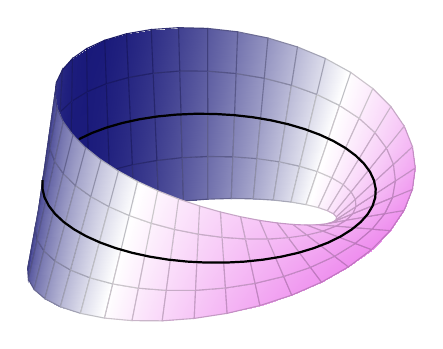
\begin{tikzpicture}
			\begin{axis}[
			  hide axis,
			  view = {40}{40}
			]
			\addplot3 [
			  surf,
			  colormap/violet,
			  shader     = faceted interp,
			  point meta = x,
			  samples    = 40,
			  samples y  = 5,
			  z buffer   = sort,
			  domain     = 0:360,
			  y domain   =-0.5:0.5
			] (
			  {(1+0.5*y*cos(x/2)))*cos(x)},
			  {(1+0.5*y*cos(x/2)))*sin(x)},
			  {0.5*y*sin(x/2)}
			);
		  
			\addplot3 [
			  samples=50,
			  domain=-145:180, % The domain needs to be adjusted manually,
							   % depending on the camera angle, unfortunately
			  samples y=0,
			  thick
			] (
			  {cos(x)},
			  {sin(x)},
			  {0}
			);
			\end{axis}
		  \end{tikzpicture}
		  \caption{Nastro di Möbius. La circonferenza disegnata serve proprio per far vedere che un giro attorno a questo nastro inverte l'orientazione: se io prendessi un versore normale "puntato" verso l'esterno, allora dopo un giro questo sarebbe invertito, dunque ci sarebbe una discontinuità e $\nu$ non sarebbe continua,
		  come richiesto dalla definizione di superficie orientabile}
	\end{figure}
\end{remark}
\begin{example}[esempio di calcolo del flusso attraverso una superficie] \hspace{1cm} \\
	Sia $T=\left\{(x, y, z) \in \mathbb{R}^3: x, y, z > 0, x + \frac{y}{2}+\frac{z}{4}=1 \right\}$ e $F(x, y, z)=(y, x, \frac{z}{2}+ y - 2)$. Calcolare il flusso attraverso questa superficie
\end{example}
\begin{proof}[Svolgimento]
	Osserviamo che, essendo il triangolo un piano "confinato" a $x, y, z > 0$, possiamo facilmente trovare il versore normale prendendo il vettore $(1, \frac{1}{2}, \frac{1}{4})$. Possiamo altrimenti porre
	$g(x, y, z) = x + \frac{y}{2} + \frac{z}{4}$ e definire il nostro triangolo tramite la funzione definente $g$: lo spazio tangente ad ogni punto $x_0$ di questa superficie sarà dato da $\nabla g(x_0) = (1, \frac{1}{2},\frac{1}{4})$. \\
	Esplicitiamo la $x$:
	$$
	x = 1 - \frac{y}{2} - \frac{z}{4} > 0 \text{ siccome } 0 < x = 1 - \frac{y}{2} - \frac{z}{4} = \varphi(y, z)
	$$
	La normale a questo piano è dato naturalmente dal gradiente che corrisponde proprio a
	$$
	\nabla g(x, y, z) = \begin{pmatrix} 
		\partial_y \varphi & \partial_z \varphi \\
		1 & 0 \\
		0 & 1
	\end{pmatrix} \implies |\nabla g| = \sqrt{(\partial_y \varphi)^2 + (\partial_z \varphi)^2 + 1} = \sqrt{1 + |\nabla \varphi|^2} 
	$$
	dunque il vettore normale è proprio
	$$
	\nu = \frac{(1, \frac{1}{2}, \frac{1}{4})}{\sqrt{1 + (\frac{1}{2})^2 + (\frac{1}{4})^2}} \implies \Phi(F, \Sigma, \nu) = \int_H \innerprod{F}{\frac{\nabla g}{\sqrt{1 + |\nabla \varphi|^2}}} \sqrt{1 + |\nabla \varphi|^2} dydz
	$$
	dove $H = \{(y, z) \in \mathbb{R}^2 : 0 < \frac{y}{2} + \frac{z}{4} < 1 \}$. Dunque
	$$
	\int_H \innerprod{F}{(1, \frac{1}{2}, \frac{1}{4})} dydz =	\int_0^2 y \int_0^{4 - 2y} dzdy = \frac{8}{3}
	$$
\end{proof}

\subsection{Frontiera regolare di un aperto}

\begin{definition}[punto regolare di frontiera e derivata esterna] \hspace{1cm} \\
	Sia $\Omega \subseteq \mathbb{R}^3$ un insieme aperto. Diremo che $x \in \text{Fr} \, \Omega$ è un punto di frontiera regolare se
	\begin{enumerate}[label=\protect\circled{\arabic*}]
		\item $\exists O \subseteq \mathbb{R}^3$ aperto tale che $x \in O \cap \text{Fr} \, \Omega$
		\item $\exists g \in C^1(O)$ tale che $O \cap \Omega = \{y \in O : g(y) < 0 \}$
		\item $\nabla g(y) \neq 0 \, \, \forall y \in O$
	\end{enumerate}
	Denoteremo con $\partial_{\text{reg}}$ la frontiera regolare o bordo regolare di $\Omega$. Diremo che $g$ definisce una porzione di frontiera regolare
	$O \cap \text{Fr} \, \Omega$ e
	$$
	\nu(y) = \frac{\nabla g(y)}{|\nabla g(y)|} \, \, \forall y \in O \cap \text{Fr} \, \Omega
	$$
	dove $\nu: \partial_{\text{reg}} \Omega \mapsto \mathbb{S}^2$ è detta normale esterna ad $\Omega$ in $x \in \partial_{\text{reg}} \Omega$.
\end{definition}
\begin{remark}
I punti regolari di frontiera sono quei punti che separano l'interno dall'esterno. Fare riferimento alla seguente immagine
\begin{figure}[H]
    \centering
    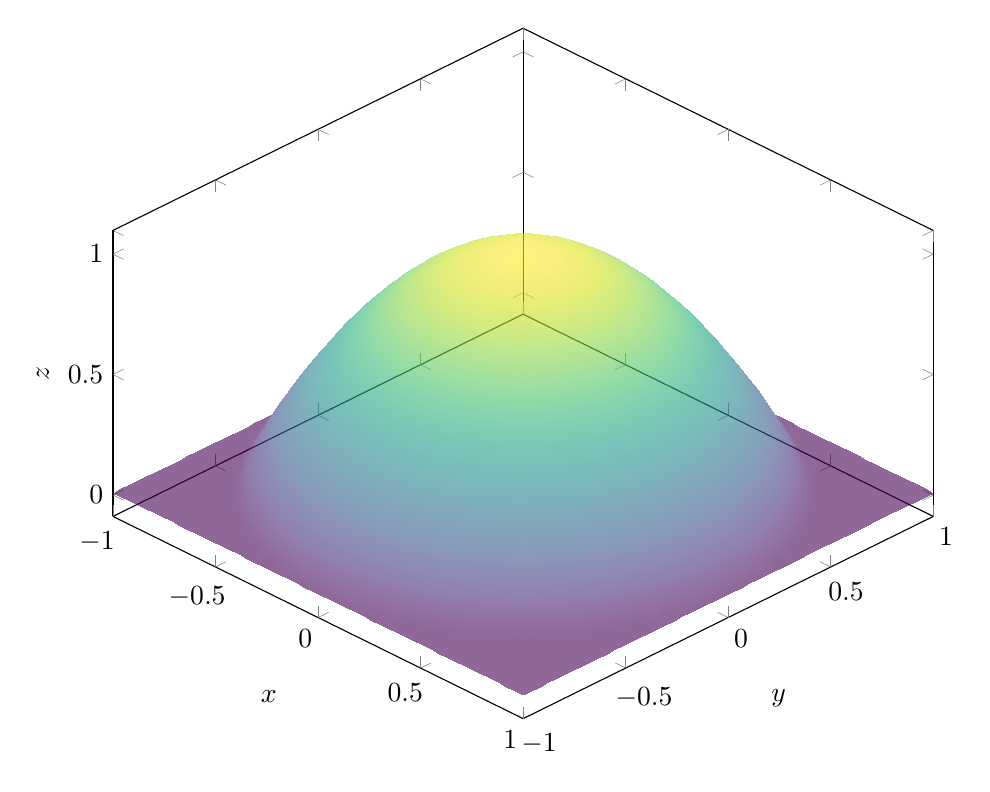
\begin{tikzpicture}
        \begin{axis}[
            width=12cm,
            view={45}{45},        % Angolazione della vista
            xlabel={$x$},         % Etichetta asse x
            ylabel={$y$},         % Etichetta asse y
            zlabel={$z$},         % Etichetta asse z
            domain=-1:1,          % Limiti degli assi x
            y domain=-1:1,        % Limiti degli assi y
            samples=50,
            clip=false,           % Disabilita il clipping
            z buffer=sort
        ]
        % Grafico della superficie limitato alla regione z > 0.01
        \addplot3[
            surf,
            opacity=0.6,          % Riduci l'opacità
            shader=interp,
            colormap/viridis,     % Sfumatura di colori più delicata
        ]
        {max(0.01, 1 - x^2 - y^2)}; % Imposta un valore minimo di z
        \end{axis}
    \end{tikzpicture}
\end{figure}
\end{remark}
\begin{prop}
	Dato $\Omega \subseteq \mathbb{R}^3$ il sottoinsieme $\partial_{\text{reg}} \Omega$ di $\text{Fr} \, \Omega$ è un'unione al più numerabile di superfici regolari.
\end{prop}
\begin{proof}[Idea della dimostrazione]
Si osserva che $\partial_{\text{reg}} \Omega$ è un'aperto in $\text{Fr} \, \Omega$ rispetto la topologia (indotta) di sottospazio e che tale topologia ha una base numerabile di aperti, dunque per il teorema di Lindelöf ogni ricoprimento aperto
ha un sottoricoprimento numerabile. Prendendo come aperti del ricoprimento di $\partial_{\text{reg}} \Omega$ gli $\{O_x : x \in \partial_{\text{reg}} \Omega \}$ dove $O_x \subseteq \mathbb{R}^3$ e $g: O_x \to \mathbb{R}$ definisce $\partial_{\text{reg}} \Omega$
intorno a $x$, dunque la tesi.
\end{proof}
\begin{prop}
Se $\nu: \partial_{\text{reg}} \to \mathbb{S}^2$ è la normale esterna allora è continua
\end{prop}
\begin{proof}
$$
\nu(y) = \frac{\nabla g(y)}{|\nabla g(y)|} \, \, y \in O \cap \text{Fr} \, \Omega
$$
è continua sulla porzione di frontiera $O \cap \text{Fr} \, \Omega$ siccome rapporto di funzioni continue
\end{proof}
Presa una funzione $F: \mathbb{R}^3 \to \mathbb{R}^3$ possiamo allora definire il flusso, supponendo che $\int_{\partial_{\text{reg}}} |F| < +\infty$ (ovvero $F$ è $\sigma-$integrale su $\partial_{\text{reg}}$), attraverso la frontiera regolare
$$
\Phi(F, \partial_{\text{reg}} \Omega, \nu) = \int_{\partial_{\text{reg}} \Omega} \innerprod{F}{\nu} d \sigma
$$
\begin{definition}[divergenza]
	Sia $F \in C^1(\Omega, \mathbb{R}^3), \Omega \subseteq \mathbb{R}^3$ aperto, allora definiamo la divergenza di $F$ la funzione scalare
	$$
	\Div F = \partial_x F_x + \partial_y F_y + \partial_z F_z
	$$
	dove $F=(F_x, F_y, F_z)$
\end{definition}
\begin{theorem}[della divergenza]
	Sia $\Omega \subseteq \mathbb{R}^3$ limitato e connesso per archi tale che
	\begin{enumerate}[label=\protect\circled{\arabic*}]
		\item $\sigma(\text{Fr} \, \Omega \setminus \partial_{\text{reg}}) = 0$
		\item $\sigma(\partial_{\text{reg}}) < +\infty$
	\end{enumerate}
	allora se $F \in C^1(\mathcal{U}, \mathbb{R}^3), \bar{\Omega} \subseteq \mathcal{U}$ dove $\mathcal{U} \subseteq \mathbb{R}^3$ è aperto vale la seguente formula
	$$
	\int_\Omega \Div F dm_3 = \int_{\partial_{\text{reg}} \Omega} \innerprod{F}{\nu} d\sigma = \Phi(F, \partial_{\text{reg}} \Omega, \nu)
	$$
\end{theorem}
\begin{example}[calcolo del flusso tramite il teorema della divergenza]
	Calcolare $\Phi(F, \Sigma, \nu)$ dove $F(x, y, z)=(x, y, z)$ e $\Sigma=\{(x, y, z) \in \mathbb{R}^3 : 4x^2 + 4y^2 + z^2 = 4, x \leq 0 \}$, dove questa è orientata dalla normale $\nu$ che è individuata dalla condizione
	$\nu(-1, 0, 0) = (-1, 0, 0)$.
\end{example}
\begin{proof}[Svolgimento]
	Osserviamo che sul semipiano $D = \Sigma \cap \{x = 0\}$ avremo che la normale $\eta = (1, 0, 0)$ mentre per quanto riguarda il resto della superficie dobbiamo essere un po' più originali.
	$$
	\Phi(F, \partial \Omega, n) = \Phi(F, \Sigma, \nu) + \Phi(F, D, \eta) \stackrel{\text{thm divergenza}}{=} \int_\Omega \Div F dm_3 = 3\int_\Omega dm_3 = 3m_3(\Omega) 
	$$
	dove $\Omega = \{(x, y, z) \in \mathbb{R}^3 | 4x^2 + 4y^2 + z^2 < 4, x < 0 \}$. Possiamo fare questo integrale senza problemi in coordinate sferiche
	$$
	m_3(\Omega) = \int_\Omega dxdydz = 2 \int_{\Omega'} dxdydz' = 2 m_3(B(0, 1) \cap \{ x < 0 \})= \frac{4}{3} \pi 
	$$
	dove, per agevolare il calcolo dell'integrale, abbiamo fatto il cambio di coordinate $(x', y', z') \mapsto (x', y', 2z') = (x, y, z)$ dunque il jacobiano di questa trasformazione era pari a $2$ e poi abbiamo diviso per $2$ per ottenere solo metà contributo della sfera (siccome la condizionee $x<0$ taglia metà della sfera).
	Dunque
	$$
	\Phi(F, \Sigma, \nu) = 3m_3(\Omega) = 4\pi
	$$
\end{proof}
Mostriamo due esempi famosi del teorema della divergenza
\subsection{Legge di Gauss}
Sia $E = k_e \frac{q}{r^2}\hat{r}$ il campo elettrico generato da una carica puntiforme, allora
\begin{align*}
&\Div E = \Div(k_e \frac{q}{r^2} \hat{r}) = \Div(k_e \frac{q}{r^3}r) = k_e q \sum_{i=1}^3 \partial_{x_i} (\frac{x_i}{|x|^3}) = k_e q \sum_{i=1}^3 \frac{|x|^3 - 3 x_i^2 |x|}{|x|^6} = \\
&=k_e q \frac{3|x|^2 - 3 |x|^2}{|x|^5} = 0
\end{align*}
$E$ è ben definito $\Omega \setminus B(x_0, \varepsilon)$ e, dunque, possiamo applicare il teorema della divergenza su $\Omega \setminus B(x_0, \varepsilon)$, da cui deduciamo che
\begin{align*}
&\Phi(E, \partial_{\text{reg}} (\Omega \setminus B(x_0, \varepsilon)), \nu) = \int_{\partial \Omega} \innerprod{E}{\nu} d\sigma + \int_{\partial B(x_0, \varepsilon)} \innerprod{E}{\nu} d\sigma = \Phi(E, \partial \Omega, \nu) - k_e \frac{q}{\varepsilon^2} (4 \pi \varepsilon^2) = \\
&=\int_{\Omega \setminus B(x_0, \varepsilon)} \Div E dm_3 = 0 \implies \Phi(E, \partial \Omega, \nu) = 4 \pi k_e q
\end{align*}
dove abbiamo usato il fatto che $\int\limits_{B(x_0, \varepsilon)} \innerprod{E}{\nu} = E 4 \pi \varepsilon^2$ in virtù delle simmetria radiale del campo elettrico.
\subsection{Equazione di continuità in fluidodinamica}
Sia $\Omega$ una regione di spazio di un fluido che sta "uscendo" da questo e indichiamo con $d\Sigma$ l'elemento infinitesimo di superficie, $d\sigma$ l'elemento infinitesimo di area e $v(x, y, z, t)$ la velocità della particella di un liquido nel punto $(x, y, z)$ al tempo $t$. In un tempo
infinitesimale $dt$, l'elemento infinitesimale di volume di liquido passante attraverso l'elemento di superficie $d\Sigma$ è pari a $|\vec{v} \cdot \nu|d\sigma$, dove $\vec{v}$ è la velocità del liquido mentre $\nu$ è la normale alla
superficie. Supponendo che il nostro liquido abbia una densità $\rho(x, y, z, t) \geq 0$ variabile, la quantità di fluido totale è data da
$$
V = \int_\Sigma \rho (\vec{v} \cdot \nu)d\sigma = \Phi(\rho \vec{v}, \Sigma, \nu) 
$$
Per la conservazione della massa dobbiamo avere che
$$
\frac{M_t - M_{t+dt}}{dt} = V
$$
ma sapendo che $M_t = \int\limits_\Omega \rho(x, y, z, t) dxdydz$ (ovvero la massa di tutto il fluido è l'integrale in tutta la regione di spazio $\Omega$ in cui si trova il fluido al tempo $t$), allora
$$
-\frac{\partial}{\partial t} \int_\Omega \rho(x, y, z, t)dxdydz = \int_{\partial \Omega} \rho \vec{v} \cdot \nu d\sigma
$$
dove il $-$ deriva dal fatto che la $V$ è naturalmente positiva ma il bilancio di massa dove che il fluido esce dalla superficie diminuisce, dunque la derivata è negativa. Tramite la teoria di Lebesgue è possibile portare la derivata all'interno dell'integrale con ipotesi deboli, dunque
$$
\int_\Omega - \frac{\partial \rho}{\partial t} dm_3 = \Phi(\rho \vec{v}, \partial \Omega, \nu) \stackrel{\text{thm divergenza}}{=} \int_\Omega \Div(\rho \vec{v}) \implies \frac{\partial \rho}{\partial t} + \Div(\rho \vec{v}) = 0
$$
che prende il nome di equazione di continuità.

\section{Teorema del rotore}

Vogliamo adesso enunciare il teorema del rotore. Ci limiteremo all'enunciato relativo alle superfici elementari, ma naturalmente è possibile mostrare la sua valenza anche per superfici più "generali". Prima di fare ciò è necessaria e, soprattutto, doverosa qualche definizione.

\subsection{Superfici elementari}

\begin{definition}[curva regolare a tratti]
	Una curva $\gamma: [a, b] \to \mathbb{R}^n$ si dice regolare a tratti se $\gamma \in C^1_\text{tratti}$ e $\dot{\gamma}(t) \neq 0 \, \, \forall t \in (t_{i-1}, t_i) \, \, \forall i \in \{1, \ldots, N \}$ dove $a=t_0 < t_1 < \ldots < t_{N-1} < t_N = b$ è il partizionamento che rende $\gamma$ $C^1_\text{tratti}$. Se $N=1$, ovvero $t_0=a$ e $t_1=b$ diremo che $\gamma$ è regolare.
\end{definition}
\begin{definition}[dominio piano elementare]
	Un insieme $H \subseteq \mathbb{R}^2$ è detto dominio piano elementare se è limitato e la sua frontiera $\partial H$ è una curva semplice, chiusa e regolare a tratti 
\end{definition}
\begin{remark}
Il "bordo" di questo dominio può essere frastagliato in alcuni punti
\begin{figure}[H]
	\centering
	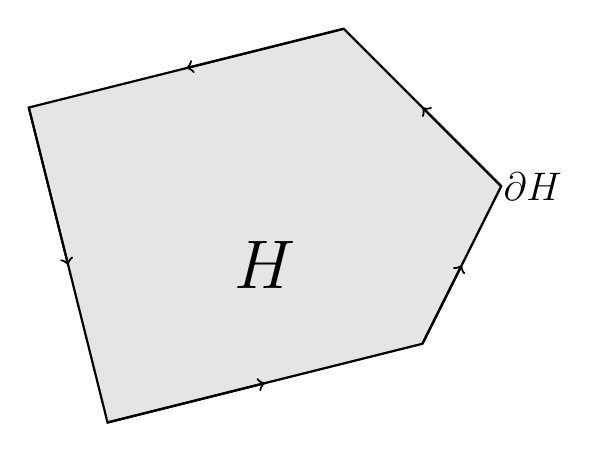
\begin{tikzpicture}[scale=2]
		\filldraw[fill=gray!20, draw=black, thick] 
			(0, 0) -- (2, 0.5) -- (2.5, 1.5) -- (1.5, 2.5) -- (-0.5, 2) -- cycle;
		
		% Etichetta della regione H
		\node at (1, 1) {\Huge $H$};
	
		% Disegna la frontiera con frecce per l'orientamento
		\draw[->, thick] (0, 0) -- (1, 0.25);
		\draw[->, thick] (2, 0.5) -- (2.25, 1);
		\draw[->, thick] (2.5, 1.5) -- (2, 2);
		\draw[->, thick] (1.5, 2.5) -- (0.5, 2.25);
		\draw[->, thick] (-0.5, 2) -- (-0.25, 1);
	
		% Etichetta della frontiera
		\node at (2.7, 1.5) {\Large $\partial H$};
	
		% Disegna una curva rossa tra due punti adiacenti sulla frontiera
		%\draw[thick, red] (2, 0.5) to[out=120, in=240] (2.5, 1.5);
	
		% Punti di partenza e arrivo della curva
		%\filldraw[red] (2, 0.5) circle (0.05);   % Punto iniziale
		%\filldraw[red] (2.5, 1.5) circle (0.05); % Punto finale
	
		% Aggiungi un clip per evitare che il riempimento si estenda oltre la curva rossa
		\clip (0, 0) -- (2, 0.5) -- (2.5, 1.5) -- (1.5, 2.5) -- (-0.5, 2) -- cycle;
	\end{tikzpicture}
	\caption{Esempio di dominio piano elementare. Come si vede il bordo è frastagliato, eppure è possibile parametrizzare il bordo con una curva semplice, chiusa e regolare a tratti}
\end{figure}
\end{remark}
Tramite i domini elementari possiamo definire le superfici elementari
\begin{definition}[superficie elmentare]
	Diremo che $\Sigma \subseteq \mathbb{R}^3$ è una superficie elementare se esiste un dominio piano elementare $H \subseteq \mathbb{R}^2, \mathcal{U} \subseteq \mathbb{R}^2$ aperto e una funzione $\Phi: \bar{H} \to \mathbb{R}^3$ tali che
	\begin{enumerate}[label=\protect\circled{\arabic*}]
		\item $\Phi$ è iniettiva su $\bar{H}$, $\bar{H} \subset \mathcal{U}$, $\Phi \in C^1(\mathcal{U}, \mathbb{R}^3)$;
		\item $d\Phi: \mathbb{R}^2 \to \mathbb{R}^3$ è iniettivo $\forall u \in \bar{H}$;
		\item $\Sigma = \Phi(H)$.
	\end{enumerate}
	Inoltre, diremo che $\Phi$ è una parametrizzazione di $\Sigma$, $\bar{\Sigma} = \Phi(\bar{H})$ è la chiusura di $\Sigma$ pertanto, posto $\partial \Sigma = \Phi(\partial H)$, avremo che
	\begin{equation}
		\bar{\Sigma} = \Sigma \cup \partial \Sigma
	\end{equation}
\end{definition}
\begin{remark}
	La condizione $\Phi(\partial H) = \partial \Sigma$ serve per evitare delle situazioni come il grafico dell'\emph{otto}: possiamo parametrizzare un $8$ solo per $y>0$ ma in $z=0$, se invertiamo la funzione localmente, possiamo estenderla anche al semipiano inferiore ottenendo qualcosa che non è più un $(x, y)-$grafico.
\end{remark}
\begin{remark}
Possiamo mostrare che una superficie elementare è una superficie regolare, siccome $\Sigma$ è localmente un grafico. Infatti
$$
D\Phi(u) = \begin{pmatrix}
\nabla \Phi_1(u) \\
\nabla \Phi_2(u) \\
\nabla \Phi_3(u)
\end{pmatrix}
$$
e supponiamo che $M_{\text{12}}(D\Phi) = \det \begin{bmatrix} \nabla \Phi_1 \\ \nabla \Phi_2 \end{bmatrix} \neq 0$: possiamo considerare $\Phi_{(1, 2)}: U \to \mathbb{R}^2$ tale che $u \mapsto (\Phi_1(u), \Phi_2(u))$. Per ipotesi avremo che $\det D\Phi_{(1, 2)}(u) = M_{12}(D\Phi(u)) \neq 0 \implies$ per il teorema della funzione inversa $\exists \delta > 0: \exists V \subseteq \mathbb{R}^2: \Phi_{(1,2)}: B(u, \delta) \to V$ invertibile con inversa $\Psi: V \to B(u, \delta) \in C^1(V, B(u, \delta))$.
Ma allora $(\Phi \circ \Psi)(u) = (\Phi_1(\Psi(v)), \Phi_2(\Psi(v)), \Phi_3(\Psi(v))) = (\Phi_{(1,2)}(\Psi(v)), \Phi_3(\Psi(v))) = (v, \Phi_3(\Psi(v)))$ siccome $\Psi = \Phi_{(1,2)}^{-1}$. A questo punto possiamo localmente vedere questa superficie elementare come quella che soddisfa l'equazione $z = \Phi_3(\Psi(v))$ e, ponendo $g = \Phi_3 \circ \Psi$, avremo la seguente equazione definente $z=g(v) \implies z - g(v) = 0 \implies \Sigma=f^{-1}(0)$ dove $f(v, z) = z - g(v)$. \\
\end{remark}
Le superfici elementari "non hanno buchi", ovvero sono degli insiemi semplicemente connessi: consideriamo una curva $\gamma: [a,b] \to \Sigma$ chiusa, allora possiamo considerare la composizione $\Phi^{-1} \circ \gamma : [a, b] \to \bar{H}$ e, siccome $\Phi$ è iniettiva su $\bar{H}$, avremo che la curva $\Phi \circ \gamma$ è anch'essa una curva chiusa. Ma allora sappiamo che $\exists x_0 \in \bar{H} : \exists \mathcal{H} : [0, 1] \times [a, b] \to \bar{H} : \mathcal{H}(0, \cdot) = \Phi^{-1} \circ \gamma(\cdot), \mathcal{H}(1, \cdot) = x_0$, da cui si deduce che
la funzione $\Phi \circ \mathcal{H} : [0, 1] \times [a, b] \to \Sigma$ è una funzione continua tale che $\Phi \circ \mathcal{H}(0, \cdot) = \gamma(\cdot), \Phi \circ \mathcal{H}(1, \cdot) = \Phi(x_0)$ e $\forall t, \mathcal{H}(t, a) = \mathcal{H}(t, b) \implies \Phi \circ \mathcal{H}(t, a) = \Phi \circ \mathcal{H}(t, b)$ per l'iniettività di $\Phi$. La funzione $\Phi \circ H$ è allora è un'omotopia di $\gamma$ in $\Phi(x_0)$.

\begin{prop}
	Se $\gamma \in C^1(\mathcal{U}), \mathcal{U} \subset \mathbb{R}^2$ aperto, $H \subset \mathbb{R}^2$ è un dominio piano elementare e $\bar{H} \subset \mathcal{U}$, allora $\Phi(x, y) = (x, y, \varphi(x, y)), (x, y) \in \mathcal{U}$ definisce una superficie regolare $\Sigma = \Phi(\mathcal{U})$ che è il grafico di $\varphi$ su $\mathcal{U}$.
\end{prop}
\begin{proof}
Osserviamo banalmente che le condizioni $\circled{1}$, $\circled{2}$ della definizione di superficie regolare sono verificate, mentre l'ultima condizione segue da come è stata definita $\Sigma$.
\end{proof}
\begin{remark}
	E' facile osservare che la proposizione $1$ si può formulare analogamente per i casi in cui $\Phi(x, z) = (x, \varphi(x, z), z), (x, z) \in \bar{H}$ e $\Phi(y, z) = (\varphi(y, z), y, z), (y, z) \in \bar{H}$.
\end{remark}
Possiamo a questo punto definire il concetto di normale esterna
\begin{definition}[normale esterna]
	Sia $H \subseteq \mathbb{R}^2$ aperto un dominio piano elementare e sia $\gamma : [a, b] \to \partial H$ una curva semplice, chiusa e regolare a tratti rispetto a $a = t_0 < t_1 < \leq < t_k = b$ la cui immagine è il bordo $\partial H$. Possiamo inoltre assumere che $\gamma$ orienti la curva positivamente, ovvero 
	percorre $H$ lasciandolo a sinistra. Definiamo la normale esterna come
	\begin{align*}
	&\eta(\gamma(t)) = \frac{R\dot{\gamma}(t)}{|R\dot{\gamma}(t)|} & &\forall t \in (t_{j-1}, t_j) \, \forall k \in \{1, \ldots, k \}
	\end{align*}
	dove $R$ è la matrice di rotazione $\frac{\pi}{2}$ in senso orario.
\end{definition}
\begin{figure}[H]
	\centering
	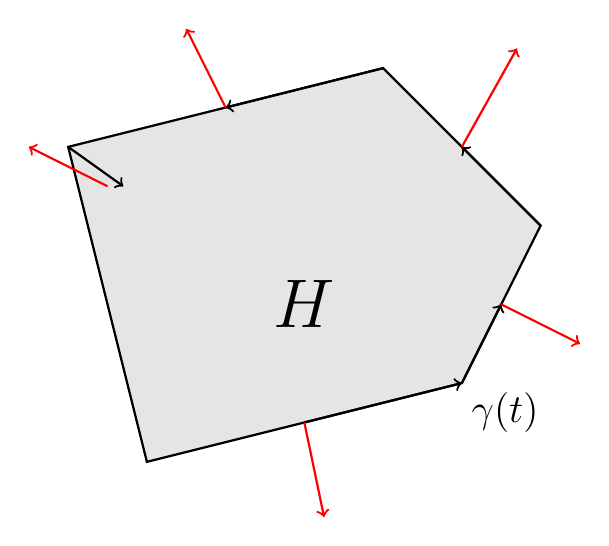
\begin{tikzpicture}[scale=2]
		% Regione H
		\filldraw[fill=gray!20, draw=black, thick] 
			(0, 0) -- (2, 0.5) -- (2.5, 1.5) -- (1.5, 2.5) -- (-0.5, 2) -- cycle;

		% Etichetta della regione H
		\node at (1, 1) {\Huge $H$};

		% Frontiera con frecce per l'orientamento
		\draw[->, thick] (0 + 1, 0+0.25) -- (1+1, 0.25+0.25);
		\draw[->, thick] (2, 0.5) -- (2.25, 1); 
		\node[anchor=north west] at (2, 0.5) {\Large $\gamma(t)$};
		\draw[->, thick] (2.5, 1.5) -- (2, 2);
		\draw[->, thick] (1.5, 2.5) -- (0.5, 2.25);
		\draw[->, thick] (-0.5, 2) -- (-0.15, 1.75);

		% Vettori normali esterni ortogonalizzati
		\draw[->, red, thick] (1, 0.25) -- (1.125, -0.35); % Normale esterna in basso (rotazione 90°)
		\draw[->, red, thick] (2.25, 1) -- (2.75, 0.75);  % Normale esterna a destra
		\draw[->, red, thick] (2, 2) -- (2.35, 2.625);    % Normale esterna in alto a destra
		\draw[->, red, thick] (0.5, 2.25) -- (0.25, 2.75); % Normale esterna in alto a sinistra
		\draw[->, red, thick] (-0.25, 1.75) -- (-0.75, 2);  % Normale esterna a sinistra

		% Clip per mantenere il riempimento
		\clip (0, 0) -- (2, 0.5) -- (2.5, 1.5) -- (1.5, 2.5) -- (-0.5, 2) -- cycle;
	\end{tikzpicture}
	\caption{(Da sistemare): normale esterna nel caso di un dominio piano elementare}
\end{figure}

Consideriamo adesso $\Phi: U \to \mathbb{R}^3$ di classe $C^1$ una parametrizzazione di una superficie elementare $\Sigma = \Phi(H)$ e $H$ un dominio piano elementare. Abbiamo visto dal capitolo \ref{cap:curve_superfici_regolari} che preso $p \in \Sigma$ con $p = \Phi(w), w \in H$ allora abbiamo che lo spazio tangente a $\Sigma$ in $p \in \Sigma$ è dato da
$$
	T_p(\Sigma) = \text{Span}{\partial_1 \Phi(w), \partial_2 \Phi(w)}
$$
mentre una normale a $\Sigma$ in $p$ è data da
$$
	\nu(p) = \frac{\partial_1 \Phi(w) \times \partial_2 \Phi(w)}{|\partial_1 \Phi(w) \times \partial_2 \Phi(w)|}.
$$
Possiamo dunque orientare una superficie elementare scegliendo sempre il campo normale
$$
\nu(p) = \frac{\Phi_{u_1} \Phi(\Phi^{-1}(p)) \times \Phi_{u_2} (\Phi^{-1}(p))}{|\Phi_{u_1} \Phi(\Phi^{-1}(p)) \times \Phi_{u_2} (\Phi^{-1}(p))|}
$$
\newpage 
\newpage 
\newpage